\documentclass[hidelinks, a4paper,12pt]{article}

\usepackage{graphicx}
\usepackage{amsmath,amssymb,amsthm} 
\usepackage[toc,page]{appendix}
\usepackage{longtable,rotating,subcaption}
\usepackage[margin=3cm]{geometry}
\usepackage{natbib}
\usepackage{multicol}
\usepackage[pdftex,hypertexnames=false,linktocpage=true]{hyperref}
\usepackage[dvipsnames]{xcolor}
\usepackage{chngcntr}
\usepackage{cleveref}
\usepackage{lscape}
\usepackage{subcaption}
\usepackage{tikz}
\usepackage{everypage}
%\usepackage[nottoc,numbib]{tocbibind}

\counterwithin{figure}{section}
\counterwithin{equation}{section}
\counterwithin{table}{section}

\usepackage{natbib}
\usepackage[section]{placeins}
\usepackage{filecontents}
\urlstyle{same}

\renewcommand{\baselinestretch}{1.1}
\newcommand{\multlinecomment}[1]{\directlua{-- #1}}

\title{Multi step forecasting with machine learning and statistical models}
\author{
    Michiel B.\ van den Engel
    (VU Student Number: 2612085)
    \\[2ex]
    Supervisor: Ilka\ van de Werve\\
    }
\date{Autumn 2022}

\newlength{\hfoot}
\newlength{\vfoot}
\AddEverypageHook{\ifdim\textwidth=\linewidth\relax
\else\setlength{\hfoot}{-\topmargin}%
\addtolength{\hfoot}{-\headheight}%
\addtolength{\hfoot}{-\headsep}%
\addtolength{\hfoot}{-.5\linewidth}%
\ifodd\value{page}\setlength{\vfoot}{\oddsidemargin}%
\else\setlength{\vfoot}{\evensidemargin}\fi%
\addtolength{\vfoot}{\textheight}%
\addtolength{\vfoot}{\footskip}%
\raisebox{\hfoot}[0pt][0pt]{\rlap{\hspace{\vfoot}\rotatebox[origin=cB]{90}{\thepage}}}\fi}


\graphicspath{ {./pics/} }

\begin{document}
\maketitle

\begin{abstract}
\noindent In this thesis, we implemented multiple machine learning and statistical methods on German and Dutch customer service data and tested these models on multiple time horizons, tested the significant differences and concluded that the ARIMAX and regression model for Dutch and German Data had the best performance.\\[1ex]
\noindent\textbf{Key words: } XGBoost, VARIMAX, Fused Lasso, Machine Learning, Statistical Models, Neural Network, Diebold Mariano. 
\end{abstract}

\vfill
\centerline{
\includegraphics[width=0.5\textwidth]{picnic_auto.png}}
\vfill
\centerline{
\includegraphics[width=0.5\textwidth]{VU_logo.jpg}}
\clearpage
\tableofcontents
\newpage
\section{Introduction}
For a multi-step ahead forecast, there are many different models that a data scientist might use. Many models have different advantages and disadvantages and might be better or worse for a specific situation. Most forecasting models can be classified in one of two different categories: machine learning models and statistical models. In this thesis we will look at these models and research if they perform differently on multi-step ahead forecasts.\\

Time series models have a lot of applications, from the prediction of sales \citep{Pavlyshenko2019Machine-LearningForecasting} to proving that the climate crisis is caused by humans \citep{Stern2013AnthropogenicChange}. For this wide range of applications it is important to research the performance of the methods used by researchers. For example \cite{Crane-Droesch2018MachineAgriculture} uses forecasting methods to predict the impact of climate change to the agricultural output from the US midwest. In this thesis we will focus on the application of multi-step forecasting. The models we use can be broken up in two categories: the statistical methods and the machine learning methods. We compare models from these two categories on 7 step (one week), 28 step (four weeks) and 49 step (seven weeks) horizons and we will research if there is a difference in performance of these models on these horizons.\\

One of the studies that compare multiple machine learning models and statistical is done by \cite{Papacharalampous2019ComparisonProcesses} who compare different statistical models and machine learning models for hydrological processes. \cite{Papacharalampous2019ComparisonProcesses} find that for hydrological processes the machine learning models and statistical models do not differ much in performance. In this thesis we will expand the existing literature by adding results for a completely different process. \cite{Alon2001ForecastingMethods} compare an Artificial Neural Network to a more traditional ARIMA model on multi-step forecasting performance and concludes that the Machine Learning Model has a better performance. In this thesis we do this comparison not only for the ARIMA model and the Neural Network, but also for some expanded statistical methods, a tree structured machine learning model and for models that use a multivariate breakdown of the data.\\

To add to the literature we will train ten different models and then test with the Diebold-Mariano test if the forecasts produced by these models are significantly statistically different. The statistical models we will train and compare are the local level model, the regression model, the ARIMA model, the ARIMAX model, the VARIMAX model, the Fused Lasso model, and the machine learning models are the XGBoost model, a Neural Network and a multivariate Neural Network. Lastly, we will also create a mixed model which is an aggregate of two statistical and two machine learning models. With these models, we do not find any evidence that the machine learning models perform significantly better than the statistical methods and we also find that for the two different data sets used, there is no one method that performs the best on both the data sets.\\

To test these models we will make use of data from the Picnic customer service department. Picnic is an online supermarket startup which operates in the Netherlands, Germany and France.  With this data, we make a forecast for each of the 10 proposed models and determine which will conclude that the method which predicts the total number of cases best is the ARIMAX model. A customer service case can be anything where a customer service agent needs to take a look at. Most cases have come from whatsapp or feedback (where a customer can give feedback in the app for the delivery), but they can also come in from delivery drivers, phone calls, email and social media. These cases are all classified with certain skill types that are correspond with training agents can do.\\

We will compare the ten individual models We will give a general description of how all of these models work in \autoref{seq:methodology}. We will describe what data we will use for the model estimations to give an understanding of the context in which this comparison is done in \autoref{seq:the data}. We will report the forecast results and estimated parameters of all statistical models and we will perform statistical tests to check if the difference in performance is significant which are described in \autoref{seq:results}. Finally, in \autoref{seq:conclusion} the findings of this thesis are described.

%Most large companies employ a customer service team. These teams solve any issues that customers might have. An agent at a customer success team answers messages coming from customers and helps the customers with issues they might have. If an issue comes in, the customer success systems create a case and the case will be handled by an agent. Cases can come in via different ways, like WhatsApp, Phone, Feedback in the app, Mail and more. If there are too few agents at work, the waiting times will increase and customers will leave the queue. \citep{Zohar2002AdaptiveSupport}\\

%The negative effect of queues is not only seen at customer service operations, but also in restaurants \citep{DeVries2018WorthRevenue}, stores \citep{Lu2013MeasuringPurchases} and physical help desks \citep{Zhou2003LookingBehind}. \cite{Lu2013MeasuringPurchases} concludes that customers are heterogeneous in their sensitivity to queues. The effects of too long queues cannot easily be understated as \cite{Bielen2007WaitingServices} find that the level of satisfaction with the customer service experience impacts the level of customer loyalty. \cite{Davis1998HowSatisfaction} show that the impact of the actual waiting time on customer satisfaction has an increasing influence as the waiting time increases.\\

%At every customer service operation there is a balance to achieve. As there are more agents working the waiting time for customers will decrease, but this costs the company a lot of money \citep{Liu2017InfluenceCenters} and if there are too many agents working, they might not have any cases left and cannot work effectively. To make sure the waiting times keep to a minimal while the resources of the company are not wasted a reliable forecast is needed.\\

%Therefore we want to make a forecast for the number of incoming cases in the customer success operations at the customer service of the Picnic supermarket. We want to look at different models and see what model performs the best. We will compare Machine learning and statistical methods of forecasting and report the quality measures of these methods.\\

%Making a forecast for a customer service operation is notoriously challenging as the number of incoming cases is highly volatile \citep{Hafeez2013PlanningLevels}. The number of customers might increase due to incidents that cannot be taken into account in a forecast model. A situation like this at Picnic in August 2022 there was an issue with dry ice which had as a result that customers could not order any frozen products resulting in an increase of the cases per delivery.\\

%The business at the moment has three main stakeholders, the recruitment team, the long term planner and the short term planner. From past experience however, we learn that if a forecast is available, more applications of the forecast can be discovered. The three main use cases that would start using the forecast immediately are:
%\begin{enumerate}
%    \item The recruitment for customer service team needs to make a correct assessment about the number of agents in service and how many agents should be hired. This information is needed months into the future for a stable hiring program as new agents need to be found and trained.
%    \item A customer service planner is also benefited by this forecast as the planner needs to make sure there are enough agents but for this purpose it is required to make a forecast that goes far into the future making it less reliable.
%    \item Each week, the planner might look again at the planning for next week. As forecasts try to predict the future based on lagged data, the forecast will improve when the time frame moves closer to reality. There might be a shortage of planned agents due to agents quitting and or forecast adjustments and the operations might want to ask agents to work extra and possibly add extra benefits for agents to do extra work.
%\end{enumerate}
%As described above there are multiple use cases for this forecast. This results in some problems with making the forecast. The forecast is used at the intervals of 1 week, 4 weeks and 7 week intervals. These used cases might benefit from different trained models and in this Thesis we will compare multiple models on different time intervals and see if a time varying combination of these models might perform better over different time periods.
\section{Literature Review}
The aim of this thesis is to compare forecasts over different time horizons, to look if some methods might have a better performance on different horizons and compare different forecasting methods to each other. Overall, the focus will be on a multi step forecast as this is in practice the most used application of forecasting models.

\subsection{Multi-step Forecasting}
%Different forecasts and multiple horizons
A problem that often arises when making multi-step forecasts is that of accumulation errors. A typical forecast uses the predictions made of previous data points in the forecast for the next data points \citep{Chevillon2007DirectForecasting}.\\

The importance of the multi-step ahead forecast is hard to overstate, as it is vital for many businesses, as businesses become more data driven. However, most research in forecasting is done on the one-step ahead forecasting \citep{Duan2021LearningForecasting}. In this thesis we want to compare a number of different forecasting methods for our data sets on different time horizons.\\

% Add something about why and that combining may make this better

Among with trying different forecasting methods, we will also try to improve these forecasting methods by combining a diverse range of forecasting methods to a mixed model. This concept is well studied \citep{Amstrong2001CombiningForecasts, Stock2004CombinationSet} since \cite{Bates1969TheForecasts} showed that combining the data points of two forecasts to one forecast results in a lower mean squared error. In the more recent past, \cite{Yang2004CombiningResults} builds on the result by \cite{Bates1969TheForecasts} and creates a more general theoretical framework for combining forecasts. These combined models can work as a safeguard for a too narrow specified model if the framework is diverse enough \citep{Amstrong2001CombiningForecasts}.\\

%Using the combination of forecasts in a different way, \cite{Engle1989MergingForecasting} describes a combination of models where a model is made over a short and long term horizon and then combined. This concept is then expanded by \cite{Andrawis2011CombinationForecasting} who combines two forecasting models into a short-long term model and concludes that the different time scales taken into account makes sure that the different dynamics of the time scales are better reflected into the final model which in turn will result in a better forecast.\\

% Add something about the benefits of sort-long term modeling circling back to the first part

% Interval difference
An example of this is the research that has been done by \cite{Ringwood2001ForecastingNetworks}  who compare a linear model and a neural network to model three different time scales on hourly, weekly and yearly intervals. They find that the neural network in general outperforms the linear model over all the time intervals.\\

\subsection{Machine Learning and statistical methods comparison}
% The beef
There have been some studies at comparing machine learning models to traditional statistical models in general. \cite{Makridakis2018StatisticalForward} write about the best practices and errors that were made in the past as well as doing a wide comparison themselves. The result from their own research is that the traditional statistical models outperform the machine learning models in general, although they note that this might be because of their specific data set and because of that more research is needed. \cite{Makridakis2018StatisticalForward} also note that there needs to be more research comparing machine learning models with traditional statistical models \citep{Chatfield1993NeuralFad}.\\

Another improvement to the current literature could be made by applying statistical tests when comparing forecasts of machine learning methods comparisons with the forecasts of traditional statistical methods \citep{Masini2021MachineForecasting, Makridakis2018StatisticalForward}. This is not always done correctly as \cite{Adya1998HowEvaluation} showed when they did a meta study of 48 studies and found that only eleven of these studies did correct validations. For this thesis the importance of a good comparison metric cannot easily be understated. A meta analysis done by \cite{Peng2014APractice} suggests that studies comparing forecast models should at least report some error measures MAPE and RMSPE. It is also suggested to add even more error measures for even more complete results.\\

% our models compare between machine learning and regression
Since the time of \cite{Adya1998HowEvaluation}, a number of other studies have been undertaken to fill the hole in the literature on comparing machine learning models with traditional statistical methods. The literature has many studies comparing models to ARIMA, but there are fewer studies comparing other models with non-ARIMA models. \cite{Siddikur2022AccuracyBangladesh} compared the ARIMA model to the XGBoost model with respect to short-term Covid-19 data and found that the ARIMA model slightly outperforms the XGBoost model while \cite{Alim2020ComparisonStudy} found that XGBoost outperforms ARIMA for predicting the seasonality of brucellosis in mainland China.\\

\cite{Comrie2012ComparingForecasting} compared a neural network against a typical multivariate linear regression and concluded that the neural network performs slightly better. \cite{Mitrea2009AStudy} came to the same conclusion but also noted that a traditional forecasting method might perform better if the training data is limited in number.\\

%The state space models are compared to the ARIMA model by \cite{Ramos2015PerformanceForecasting} who concludes that state space models have a higher forecasting accuracy than the ARIMA model.\\

As seen above, many of the papers comparing the machine learning models and traditional statistical models do not focus on the difference in performance over different horizons but only compare forecasts produced by the methods on a one-step-ahead prediction error \citep{Rafael2019EvaluationModel}. It can further be seen that the current literature has no coherent conclusions for the best model in a given situation. This is very specific to the situation and the goal of this thesis is to research how these models behave in a customer success environment where everything in the organisation can have a predicting effect on cases. 
\section{Methodology}
\label{seq:methodology}
In this thesis we will compare ten models to each other for three different time intervals. The models we choose are diverse in the way they work to make better comparisons.\\

We start with one of the most basic statistical methods there is, the Local Level model described in \ref{subsec:state space}. This model tries to explain the data with a local average. Then we add regressor data to the local level model resulting in the regression model, also described in \autoref{subsec:state space}. To place this thesis better in the literature we will also make an ARIMA model described in \autoref{subsec:arima} as many research exists comparing models to the ARIMA model. As with the Local Level model, we can expand the ARIMA model with regressor data resulting in the ARIMAX model described in \autoref{subsec:arimax}. The Fused Lasso model introduces some temporal awareness and shrinks regressors that are far away from each other in time which we think would be a valuable addition to the already listed models. The fused lasso is further described in \autoref{subsec:flasso}. The two univariate machine learning models we will use are the Artificial Neural Network and extreme gradient boosting models. The Artificial Neural Network uses a Neural Network to model non-linear relationships described in \autoref{subsec:ann} and the XGBoost model constructs a decision tree to make predictions described in \autoref{subseq:xgb}.\\

There are also two multivariate models that use data which is split by skill which is needed to solve the case. These skills correspond with specific training an agent can do to acquire certain skills.To compare the multivariate models with the univariate models, the predictions for the different case types are added together such that we again get the total number of cases from the multivariate models. The underlying assumption is that the multivariate models can discover more patterns in the data and can possibly perform better than their univariate counterparts. To model this we introduce two more models, the statistical VARIMAX model (further described in \autoref{subsec:varimax}) that is a multivariate version of the ARIMAX model, and a multivariate version of the artificial Neural Network.\\

Introduce $t$ as the time unit of interest, with $t = 1, ..., T$, $n$ is defined as the number of regressors, with $n = 1, ..., N$. One point regressor data is defined as $x_{t, i}$, the dependent data is defined by $Y$, at point t in time it is written as $y_{t}$. The true value of a coefficient is $\beta$ while, the estimated coefficient is defined as $\hat{\beta}$. $||Z||^2_2$ is the quare of the euclidean norm of some time series Z or $\sum_{t=1}^Tz_t$.

\subsection{Local Level and Regression Model}
\label{subsec:state space}
The state space representation introduced by \cite{Kalman1960AProblems} is a model that can be represented using the two equations \eqref{eq:general_state_space} defining two variables. The observation vector $y_t$ and the state vector $\alpha_t$.  $y_t$ and $\alpha_t$ form the main parts of the state space representation. $\alpha_t$ stands for the state of the underlying model and $y_t$ is the actual result.

\begin{equation}
\label{eq:general_state_space}
\begin{aligned}
\alpha_{t+1} &= T_t\alpha_t + R_t\zeta_t \quad &\zeta_t \sim \mathcal{NID}(0, Q_t)\\
    y_t &= Z_t\alpha_t + \epsilon_t \quad &\epsilon_t \sim \mathcal{NID}(0, H_t)
\end{aligned}
\end{equation}

%\subsubsection{Kalman filter}
%\label{subsec:Kalman filter}
with parameters $T_t$, $R_t$, $Q_t$, $Z_t$, $H_t$ and $\alpha_t$ that need to be defined by the model that is represented in State Space. To update the state vector $\alpha_t$ the Kalman filter \citep{Kalman1960AProblems} can be used. The Kalman filter uses a set of equations \eqref{eq:kalman_equations} to update $\alpha_t$.

\begin{equation}
\label{eq:kalman_equations}
\begin{split}
    v_t &= y_t - Z_t a_t\\
    f_t &= Z_t P_t Z_t' + H_t\\
    K_t &= T_t P_t Z_t' F_t^{-1}\\
    a_{t+1} &= T_t a_t + K_t v_t\\
    P_{t+1} &= T_t P_t T_t' + R_t Q_t R_t' - K_t F_t K_t'\\
\end{split}
\end{equation}
With $v_t$ as the prediction error, $f_t$ as the variance of the prediction error and $K_t$ as the Kalman gain. With variance $P$ and state vector $a$ defined as:
\begin{equation*}
\begin{split}    
    a_{t+1} &= \mathbb{E}(\alpha_{t+1}|Y_t)\\
    P_{t+1} &= \mathbb{V}\text{ar}(\alpha_{t+1}|Y_t)
\end{split}
\end{equation*}
To make good estimates for our parameters, the loglikelihood is minimized using the L-BFGS-B method. The parameters which can be minimized can differ depending on the model that is represented in State Space. The loglikelihood equation is described in equation \ref{eq:kalman_loglikeli}
\begin{equation}
    \log \mathcal{L} = -\frac{n}{2} - \frac{1}{2}\sum\limits_{t=1}^n \log|F_t| - \frac{1}{2}\sum\limits_{t=1}^n v_t' F_t^{-1} v_t
\label{eq:kalman_loglikeli}
\end{equation}
Further descriptions and derivations can be found in \cite{Durbin2012TimeModels}\\
%\subsubsection{Kalman Smoother}
%An issue with the Kalman filter is that only the variables until $t$ ($[1:t]$) are taken into account and not the complete state vector $T$. This lead to results with larger differences and forecasts that do not take into account the variables that are being calculated later. The solution to this is the Kalman Smoother which uses a backward recursion on Kalman filter estimates which means that all the values $[1:T]$ are taken into account. The state smoothing algorithm is given by:
%\begin{equation}
%\begin{split}
%    L_t &= T_t - K_tZ_t\\
%    r_{t-1} &= Z_t'v_t + L_t'r_t\\
%    N_{t-1} &= Z_t'F^{-1}Z_t + L_t'N_tL_t\\
%    \alpha_t &= a_t + P_t r_{t-1}\\
%    V_t &= P_t - P_t N_{t-1} P_t\\
%\end{split}
%\end{equation}
%where we then have
%\begin{equation*}
%\begin{split}
%    \alpha_t &= \mathbb{E}(\alpha_t|Y_n)\\
%    V_t &= \mathbb{V}ar(\alpha_t|Y_n)
%\end{split}
%\end{equation*}
%Further descriptions and derivations can be found in \cite{Durbin2012TimeModels}
%}

%\subsection{Local Level Model}
The first model in state space representation that will be used in this thesis is the local level model. The local level model estimates the variance parameters of the state space vector and the state variable. The local level model gives us an idea about where the local average is. This model does not take much input parameters and can give us an idea about how a very simple model would perform in this data set as well as giving us a good starting point to start with our analysis with a model that has not many parameters. The local level model estimates the variance of the error terms as $\sigma_{\epsilon}^2$ and the variance of the state space equation $\sigma_{\eta}$. The local level model is given in state space form as:
\begin{equation}
\begin{split}
    y_t &= \alpha_t + \epsilon_t, \quad \epsilon_t \sim N(0,\sigma_\epsilon^2)\\
    \alpha_{t+1} &= \alpha_t + \eta, \quad \nu_t \sim N(0, \sigma_\eta^2)\\
\end{split}
\end{equation}
The Local level model is estimated using a Kalman Filter on the state space model with Z = 1, T = 1, R = $\sigma_\eta^2_t$, H = $\sigma_\epsilon^2$ \\

%\subsection{Regression model}
A first expansion of the local level model is to incorporate explanatory data in the model. A good explanatory data set helps the model find patters in the data which can help in making a forecast of the dependent variable. This model with explanatory data is the regression model.  The regression model can also be written in state space form. The regression model finds linear relationships between the explanatory data X and the dependent variable Y. The regression model is defined by:$$y_t = X_t\beta + \epsilon_t$$ and can be represented in state space form and estimated with a Kalman Filter as well. The state space representation of the regression model can be seen in equation \ref{eq:regression_state_space}. Where $\alpha^*$ is the new state space vector and $I_d$ is the Identity matrix.\\

\begin{equation}
    a^*_t = \left(\begin{array}{c} \beta \\ a_t \end{array} \right) \quad
    T = I_{d+1} \quad
    R = \left[\begin{array}{c} 0 \\ \sigma_\eta^2\\\end{array}\right] \quad
    Z = \left[\begin{array}{c c c c}
        x_{1,1} & \hdots & x_{1,n} &  1 \\
        \vdots &  \ddots& \vdots & \vdots \\
        x_{t,1} & \hdots & x_{t,n} & 1 \\
    \end{array}\right]
\label{eq:regression_state_space}
\end{equation}

\subsection{The ARIMA family}
Autoregressive models are models that do a 'simple' regression on their own lags. The ARIMA family of models are models based on the ARIMA (AutoRegressive Integrated Moving Average) model. Autoregressive means it regresses on the lags of the dependent variable. Integrated means it can handle integrated data and the moving average means it has a moving average component.

\subsubsection{ARIMA}
\label{subsec:arima}
The first model we want to consider from the ARIMA family is the ARIMA(p,d,q) model. This model is well studied in literature and one of the reasons we want to include this model in this thesis is that there exist many studies comparing other models we use in this thesis to the ARIMA model. To be able to better place the results of this thesis in literature the ARIMA model is included. The ARIMA model is a linear combination with lags and a moving average component. The ARIMA model assumes linear relationships of the dependent variable with its own lags. The model has p lags, is differentiated d times and has q moving average components. The ARIMA(p,d,q) model is defined in \autoref{eq:arima} with $p$ as the number of lags, $d$ as the order of differencing in the ARIMA model, q as the number of moving average components, $\bar{y}$ as the differenced value of $y$ and $\theta_j$ as the j'th moving average component with $j \in \{1, ..., q\}$.
\begin{equation}
\begin{split}
    \tilde{y}_t &= y_t - y_{t-d}\\
    \tilde{y}_t &= \sum\limits_{i=1}^p \beta_i \tilde{y}_{t-i}  + \sum\limits_{j=1}^q \theta_j \epsilon_{t-1}
\label{eq:arima}
\end{split}
\end{equation}
The parameters of the ARIMA model will be estimated using the L-BFGS-B method \citep{L-BFGS-B} to minimize the least squares function of $S_{\text{least Squares}} = \sum^n_{i=1} (Y - \hat{Y})^2$.

\subsubsection{ARIMAX}
\label{subsec:arimax}
The approaches of the ARIMA model and the regression model can be combined to form the ARIMAX model. The ARIMAX model is an extension of the ARIMA model. The full name of the ARIMAX model is the Autoregressive Integrated Moving Average with Explanatory Data. The ARIMAX model incorporates some lags of the dependent data Y and some moving average components as in the ARIMA model. The ARIMAX model differs from the ARIMA model as it incorporates a set of the explanatory data X in the model as some patterns might be explained by this data and not only from the lags. $\gamma$ represents the coefficients corresponding to the explanatory data X.\\

\begin{equation}
\begin{split}
    \tilde{y}_t &= y_t - y_{t-d}\\
    \tilde{y}_t &= \sum\limits_{i=1}^p \beta_i \tilde{y}_{t-i}  + \sum\limits_{j=1}^q \theta_j \epsilon_{t-1} + \Gamma X_t\\
    \Gamma &= \left[\begin{array}{c} \gamma_1 \\ \vdots \\ \gamma_b \end{array}\right] \quad X_t = \left[ \begin{array}{c} x_{1,t}\\ \vdots\\ x_{n,t} \end{array} \right]
\end{split}
\end{equation}
Where $b$ is the dimensionality of the explanatory data X. The ARIMA as well as the ARIMAX models are further described by \cite{Kirchgassner2013IntroductionAnalysis}. The parameters of the ARIMAX model are estimated by the L-BFGS-B method \citep{L-BFGS-B} that minimises the sum of the squared errors of the sample prediction.

\subsubsection{VARIMAX}
\label{subsec:varimax}
Because we are dealing with lags and explanatory data in this model, it might be possible to expose and describe more patterns in the data if we split the data by case skill type as a drop in temperature might have a faster or different effect on senior phone cases than on assortment suggestions. To test if this approach yields better results than directly trying to forecast the total number of cases we introduce the VARIMAX (Vector Autoregressive Integrated Moving Average with Explanatory data) model. The VARIMAX model is an extension of the ARIMA and ARIMAX models that predicts multivariate data. For the purpose of this thesis we will take the sum of the outcomes of the VARIMAX model such that we get the Total Number of Cases. The VARIMAX model is given in \autoref{eq:VARIMAX}. Because of the large number of parameters $\theta$, $\beta$ \& $\gamma$, the least squares cannot be optimized using the L-BFGS-B method, but it will be minimized instead using the SLSQP method \citep{SLSQP}.
\begin{equation}
\begin{split}
    \tilde{Y}_t &= Y_t - Y_{t-d}\\
    \tilde{Y}_t &= \sum\limits_{i=1}^p B_i \tilde{Y}_{t-i}  + \sum\limits_{j=1}^q \theta_j \epsilon_t +  \Gamma X_t\\
    Y_t &= \left[\begin{array}{c} y_{1,t}\\ \vdots \\ y_{l, t}\end{array}\right] \quad B_i = \left[\begin{array}{c} \beta_{1, i} \\ \vdots \\ \beta_{l,i} \end{array}\right] \quad \Gamma_k = \left[\begin{array}{c c c}
        \gamma_{1, 1} & \hdots & \gamma_{1, b}\\
        \vdots & \ddots & \vdots\\
        \gamma_{l, 1} & \hdots & \gamma_{l, b}\\
    \end{array}\right]\\
    X_t &= \left[\begin{array}{c c c}
        x_{1, 1, t} & \hdots & x_{1, b, t}\\
        \vdots & \ddots & \vdots\\
        x_{l, 1, t} & \hdots & x_{l, b, t}\\
    \end{array}\right]
\end{split}
\label{eq:VARIMAX}
\end{equation}
\subsection{Fused Lasso}
\label{subsec:flasso}
The fused LASSO \citep{Tibshirani2005SparsityLasso} is based on the lasso \citep{Tibshirani1996RegressionLasso}. The Fused LASSO penalises coefficients that have a large euclidean distance between each other. This might be beneficiary for a forecast as it prevents outliers and penalises large differences in the coefficients. Both the fused lasso and the lasso try to predict a linear model. The LASSO finds the coefficients with the least squared estimation: $$\hat{\beta}_{LASSO} = \min \left\{\frac{1}{T}||Y - X\beta||_2^2\right\}\quad \text{subject to} \quad \sum_j|\beta_j| \leq s_1$$
A problem with this approach is that it does not take into account temporal data. This is important as the data points close to the variables we want to predict might hold much more value than other data points. The fused lasso aims to fix this problem by introducing a new constraint to the minimisation problem which transforms the estimation to: 
\begin{equation}
\label{eq:fusedlasso}
  \begin{gathered}
    \hat{\beta}_{LASSO} = \min\limits_{\beta} \left\{\frac{1}{T}||Y - X\beta||_2^2\right\}\\
    \text{subject to} \\
    \sum_j|\beta_j| \leq s_1 \text{and} \sum^n_{j=2}|\beta_j-\beta_{j-1}|\leq s_2
\end{gathered}
\end{equation}
where $s$ is the sparsity parameter. $s_1$ penalises the regressors if they have a large value of $\beta$ which makes sure variables which contribute little to the models will receive a small value of $\beta$. $s_2$ encourages values of $\beta$ to be close to each other and penalise $\beta$'s that are far apart. The minimization problem that comes from \eqref{eq:fusedlasso} can be solved by the penalised least squared criterion. \cite{Knight2000AsymptoticsEstimators} describe the asymptotic properties for the lasso which are similar for the fused lasso. The penalised least squared criterion for the fused lasso is given in equation \eqref{eq:lassominimised} which can be minimized.
\begin{equation}
    \label{eq:lassominimised}
    \sum\limits_{i=1}^T (y_t - x_t^T\beta)^2 + \lambda^{(1)} \sum\limits^n_{j=1} |\beta_j| + \lambda^{(2)}\sum\limits^n_{j=2} |\beta_j - \beta_{j-1}|
\end{equation}
The selection of $\lambda^{(1)}$ and $\lambda^{(2)}$ is done using the leave-one-out cross-validation described in \cite{Hwang2016CrossAcceleration, Cawley2003EEcientClassifiers}

\subsection{Extreme Gradient Boosting (XGBoost)}
\label{subseq:xgb}
The first machine learning model that is included in this thesis is the XGBoost model. XGBoost is a gradient boosted tree method introduced by \cite{Chen2016XGBoost:System}. A tree method is a model that makes use of decision trees to come to a prediction. A graphical representation of a decision tree can be found in figure \ref{fig:decission_graphic} where the simple idea for a regression tree is represented with leaves and decision nodes. The XGBoost builds multiple decision trees and takes the average of these trees as the final outcome. The XGBoost has the objective to predict the outcome of
\begin{equation}
\label{eq:xgbpredictionfunc}
    \hat{y}_y = \phi(x_i) = \sum\limits_{k=1}^K f_k(x_i), \quad f_k \in \mathcal{F}
\end{equation}
where $\mathcal{F} = \{f(x)=w_{q(x)}(q:\mathbb{R}^m \to T, w \in \mathbb{R}^T)$, q maps the value to the corresponding leaf index, K is the number of additive function in the model, L is the number of leaves in the tree and $f_k$ corresponds to a leaf tree structure with leaf weights $w$. The function has no mathematical solution. Therefore the model is trained using the additive method in \eqref{eq:ministatxgboost} which penalises the outcome depending on the distance between real values and the estimated value and a regularisation term defined in \ref{eq:xgbpenalization}.
\begin{equation}
\label{eq:ministatxgboost}
\begin{gathered}
    \mathcal{L}^{(t)} = \sum\limits_{i=1}^T l(y_t, \hat{y}_t^{(t-1)} + f_t(x_t)) + \Omega(f_t)
\end{gathered}
\end{equation}
Here $l$ is a differentiable convex loss function which measures the distance between $\hat{y}_i$ and $y_i$. The $\Omega$ function penalises the model complexity and is defined in \eqref{eq:xgbpenalization}. This regularization term helps preventing overfitting and makes gives larger weights to models with a less deep tree.
\begin{equation}
\label{eq:xgbpenalization}
    \Omega(f) = \gamma L + \frac{1}{2} \lambda ||w||^2
\end{equation}
where $\lambda$ is a regularization term to avoid overfitting and $\gamma$ is the threshold parameter for adding notes such that nodes are only added to the tree if the gain is larger than $\gamma$. To be able to quickly optimize this function, the second order tailor approximation is used. The constant is removed such that the objective is simplified.
\begin{equation}
\label{eq:xgbminitailor}
    \mathcal{L}^{(t)} \approx \sum\limits_{i=1}^n[g_if_t(x_i) + \frac{1}{2}h_if_i^2(x_i)] + \Omega(f_t)
\end{equation}
with $g_i = \partial_{\hat{y}(t-1)}l(y_i,\hat{y}^{(t-1)})$ and $h_i = \partial^2_{\hat{y}(t-1)}l(y_i, \hat{y}^{(t-1)})$. Then if the structure of the tree is fixed, an optimal weight $w_j^*$ can be calculated for the leaf $j$ with
$$w_j^* = - \frac{\sum_{i\in I_j}g_i}{\sum_{i \in I_j} h_i + \lambda}$$
which has the corresponding value of 
\begin{equation}
\label{eq:xgbscorefunc}
    \tilde{\mathcal{L}}^{(t)}(q) = - \frac{1}{2} \frac{\left(\sum_{i \in I_j} g_i \right)^2}{\sum_{i \in I_j} h_i + \lambda}
\end{equation}
the value of the optimum weights for a tree in \eqref{eq:xgbscorefunc} can be used as a score function for tree $q$. However, because of computational constraints it is usually infeasible to evaluate \eqref{eq:xgbscorefunc} for all possible trees $q$. To avoid this problem, an algorithm that starts from a leaf and then adds branches is used. This algorithm then needs a split function that evaluates the split such that the algorithm can compare the splits and choose the best split. The split function used with $I = I_L \cup I_R$ is defined in \ref{eq:xgbsplitfunc}. 
\begin{equation}
\label{eq:xgbsplitfunc}
    \mathcal{L}_{split} = \frac{1}{2}\left[ \frac{\left(\sum_{i\in I_L} g_i\right)^2}{\sum_{i\in I_L}h_i + \lambda} + \frac{\left(\sum_{i\in I_R} g_i \right)^2}{\sum_{i\in I_R}h_i + \lambda} - \frac{\left(\sum_{i\in I}g_i\right)^2}{\sum_{i\in I}h_i + \lambda}\right] - \gamma
\end{equation}
The equation \eqref{eq:xgbsplitfunc} is also known as the gain function. To find the split it is not computationally feasible to use a greedy algorithm that tries every different solution. Therefore this algorithm will use the Sparsity-aware Split Finding algorithm \citep{Chen2016XGBoost:System} to build the tree.
\subsection{Artificial Neural Network}
\label{subsec:ann}

\begin{figure}
    \begin{subfigure}{.5\textwidth}
        \centering
        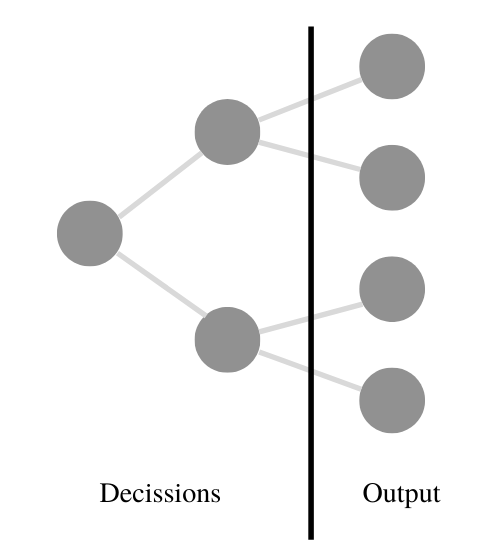
\includegraphics[width=.7\linewidth]{pics/Decission Tree.png}
        \caption{Decision tree}
        \label{fig:decission_graphic}
    \end{subfigure}%
    \begin{subfigure}{.5\textwidth}
        \centering
        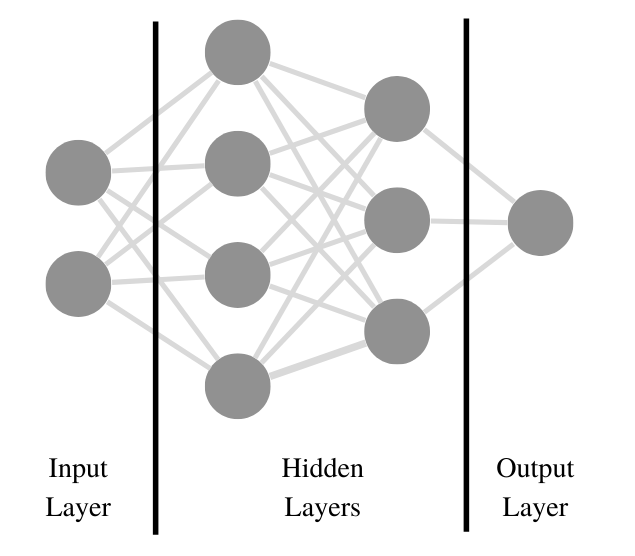
\includegraphics[width=.9\linewidth]{pics/Neural Network.png}
        \caption{Neural network}
        \label{fig:nn_graphic_representation}
    \end{subfigure}
    \centering
    \caption{A graphical representation of the models}
    \label{fig:graphical_representation}
\end{figure}

The second machine learning method we will use in this thesis is an artificial neural network. Because the neural network works in a very different way than the XGBoost model, it would diversify the selection of models in this thesis. The neural network for regression purposes was proposed by \cite{Specht1991ANetwork}. A neural network is a structure that uses one or multiple hidden layers to make a non-linear transformation which is loosely based on biological neural systems. The network consists of multiple layers performing operations and together they form the network. The three different types of layers in a neural network are the input layer, the hidden layers and the output layer. The input layer consists of the inputs $X = \{x_1, x_2, ..., x_d\}$ which are the regressors. There can only be one input layer. The hidden layers form linear combinations between the input layer, other hidden layers and the output layer. These linear combinations together will make a non-linear function. There can be multiple hidden layers. The output layer is the final layer where the dependent variables $Y = \{y_1, ..., y_d\}$ are formed. There can only be one output layer.\\

A graphical representation of these layers in a simplified form can be found in figure \eqref{fig:nn_graphic_representatio}. In this figure, one can clearly see the difference with the tree structure in \eqref{fig:graphical_representation} as there the neural network consists of multiple linear combinations combining to the answer in the end while the tree structure has multiple possible but fixed end answers. Between the layers, the function $f(x) = w_2 g(w_1^T x + b_1) + b_2$ is used. Where $\{w_1, w_2, b_1, b_2\} = \theta, w_1 \in \mathbb{R}^n \text{ and } w_2, b_1, b_2 \in \mathbb{R}$ are the function parameters. The function $g(\cdot): \mathbb{R} \to \mathbb{R}$ is the activation function defined in \eqref{eq:nn_activationfunction}
\begin{equation}
\label{eq:nn_activationfunction}
    g(z) = \frac{e^z - e^{-z}}{e^z + e^{-z}}
\end{equation}
To be able to estimate the network, backpropagation is used which tries to decrease the loss function. In every iteration, after the Loss function of the output layer is calculated, the backpropogation makes backward passes which updates the previous layers with new weights to decrease the loss function. To calculate the updated weights the L-BFGS function is used \citep{Liu1989OnOptimalization}.
\begin{equation}
    Loss(\hat{y}, y, W) = \frac{1}{2n} \sum\limits_{i=0}^n ||\hat{y}_i - y_i||^2_2 + \frac{\alpha}{2n} ||W||^2_2
\end{equation}
This thesis will use the Scikit-learn implementation of the neural model described by \cite{Pedregosa2011Scikit-learn:Python}.\\

There will also be a multivariate implementation of the neural network where the data is broken down by skill level as is also done with the VARIMAX model. The main difference of the multivariate neural network with the univariate version is that the multivariate model has multiple nodes at the output layer, resulting in a multivariate output.

\subsection{Mixed modeled Forecast}
\label{subseq:mixed model}
If we have M models $S$ which produces an output $X_s$, the output of different models $\{S_1, ..., S_n\}$ might be combined into a mixed model that outperforms all the individual models in S. In this case the mixed model $S_{\text{Mixed}}$ would look like:
\begin{equation}
    S_{\text{Mixed}}: Y_{\text{Mixed}} | X = \sum\limits_{i=1}^M \beta S_m(X)
\end{equation}
Where S is a model that produces a output Y for given data X. $\beta$ is estimated via the least squares method with X as the h ahead forecast from the selected models and Y as the true dependent. This method is shown to improve the individual forecasts that are taken into account and works better when the forecasts in $S_m$ are diverse \citep{Yang2004CombiningResults}. Because we have a lot of forecasts that are generalisations of other models, the models that will be used for this ensemble model are the Fused Lasso model, the XGBoost model, the Artificial Neural Network and the ARIMAX Model.
 
\subsection{Comparing Forecasts}
To know which forecast is the best one, we need to be able to compare them to each other. There are of course the measures of quality like MAE (Mean Absolute Error), MSE (Mean Squared Error), MAPE (Mean Absolute Percentage Error) and RMSE (Rooted Mean Squared Error) which will be computed for all the methods that are tested. The mathematical definitions of these measures of quality are described in \autoref{app:measures_of_quality}. To draw statistical significant conclusions we use the Diebold-Mariano test \citep{Diebold1995ComparingAccuracy} in combination with these benchmarks. The Diebold-Mariano test looks to evaluate the accuracy of two forecasts. Define the loss differential as: 
\begin{equation}
    d_t = g(e_{1t}) - g(e_{2_t})
    \label{eq:defferenctial_loss}
\end{equation}
Where $g(\cdot)$ is a loss function for these forecast errors which can be the MSE, MAE, MAPE, RMSE or any other information criterion. The test then seeks to verify the hypothesis defined by:
\begin{equation*}
\begin{split}
    \text{H}_0 : \mathbb{E}(d_t) &= 0 \quad \forall t\\
    \text{H}_1 : \mathbb{E}(d_t) &\neq 0 \quad \forall t\\
\end{split}
\end{equation*}
Where the null hypothesis means that the forecasts have the same accuracy while the alternative hypothesis states that the forecasts have different levels of accuracy. To construct the test statistic we need the population mean of the loss differential or:
\begin{equation*}
    f_d(0) = \frac{1}{2\pi} \left(\sum\limits_{k=-\infty}^\infty \gamma_d(k)\right)
\end{equation*}
Where $\gamma(k)$ is the autocovariance of the loss differential at lag $k$. This can be estimated with:
\begin{equation}
    \hat{f}_d(d) = \frac{1}{2\pi} \left(\hat{\gamma}_d(0) + 2 \sum\limits_{k=1}^{h-1} \hat{\gamma}_d(k)\right), \quad h > 1
\label{eq:loss_diff_hat}
\end{equation}
Where $h$ is the number of steps forecasts. By combining equations \ref{eq:defferenctial_loss} and \ref{eq:loss_diff_hat} we get the test statistic in equation \ref{eq:driebold_mariano_test_statistic} which is asymptotically N(0,1) distributed.
\begin{equation}
    DM = \frac{\bar{d}}{\sqrt{\frac{2\pi\hat{f}_d(0)}{T}}}
    \label{eq:driebold_mariano_test_statistic}
\end{equation}
\section{The Data}
\label{seq:the data}
Each model is built on a set of data and for our models this is no different. The data is provided by Picnic B.V. Picnic is an online supermarket in the Netherlands, Germany and in France. However since the operations in France are still in an earlier face, we will only focus on the Netherlands and Germany in this Thesis. Picnic maintains a high quality Data Warehouse, but since the company is still very young, only the data starting from  from 01-10-2020 until 11-11-2022 can be used. This has to do with the Picnic data being reliable from 01-10-2020 onward because at this date the Picnic customer service department fully switched to a Salesforce system for all the customer success data. This is important for the data as the Salesforce system allows for more and better quality data collection.\\

There are two databases which have the same structure. One database with data from the Netherlands and one database with data from Germany. The data from the two countries is quite different as the operations in the Netherlands are more mature. Picnic started in the Netherlands in 2015 in Amersfoort and Picnic started in 2018 in Germany in North Rhine-Westphalia.

\subsection{Data Description}
The data that is used as the dependent variable are the number of incoming cases at the customer service department. A case can come in via whatsapp, feedback via the app, email, social media or phone. These cases can be very diverse ranging from spoiled products to a customer that needs help navigating the app. From this Picnic database, we also get the number of deliveries, average Temperature and average UV index. These features standardized and plotted in figure \ref{fig:total cases NL} for the Netherlands and in figure \ref{fig:total cases DE} for Germany. In these figures the test set and the training set are represented in black and red respectively. Both data sets have large outliers at corona press conferences and national holidays. The German cases have a weakly low on Sunday as the customer service department is closed in Germany at Sundays.\\

The Picnic data is enriched with public data sources for School vacations and national holidays. This leaves us with a data set consisting of both categorical data and continuous data. The features we will use are: The first and seventh lag of the number of cases, the Number of deliveries at a certain day, the average countrywide weather temperature in Celsius, the average countrywide UV index, how many school regions have school vacation, if the day is a national holiday and lastly a unique constant for every day of the week.\\

The weather data will be different depending on the forecast horizon. This data is provided by Weather Source. For the closest horizons, we will use the weather forecasts provided by weather source. As weather forecasts are very unreliable in the further future \citep{Scher2018PredictingLearning}, the 10 year average for temperature and UV index will be used in the forecasts horizons that are further into the future.\\

The data from the school vacations comes from the Dutch Rijksoverheid website where an API exists that is used. For the German school vacations data is used from the ferien-api by Paul Brejla \citep{BrejlaDeutscheFerientermine}. For both countries the national holidays are acquired by the PyPi holidays package.\\

\begin{table}[]
    \centering
    \begin{tabular}{|c|c c c|}\hline
        Netherlands & Variance & Standard Deviation & Mean\\
        \hline
        Junior & 114222.558 & 337.968 & 1744.184\\
        Medior & 37820.469 & 194.475 & 690.138\\
        Senior & 33143.628 & 182.054 & 756.292\\
        Webcare & 189.83 & 13.778 & 19.801\\
        Assortment & 133249.88 & 365.034 & 1402.608\\
        \hline
        Germany & Variance & Standard Deviation & Mean\\
        \hline
        Junior & 199651.476 & 446.824 & 1037.731\\
        Medior & 18059.271 & 134.385 & 402.948\\
        Senior & 10507.892 & 102.508 & 190.057\\
        Webcare & 4.205 & 2.051 & 3.329\\
        Assortment & 23398.984 & 152.967 & 561.868\\\hline
    \end{tabular}
    \caption{Mean, Standard deviation and Variance and average time spend of the cases per skill level}
    \label{tab:mean_var}
\end{table}

\begin{figure}
\begin{minipage}{.5\textwidth}
  \centering
  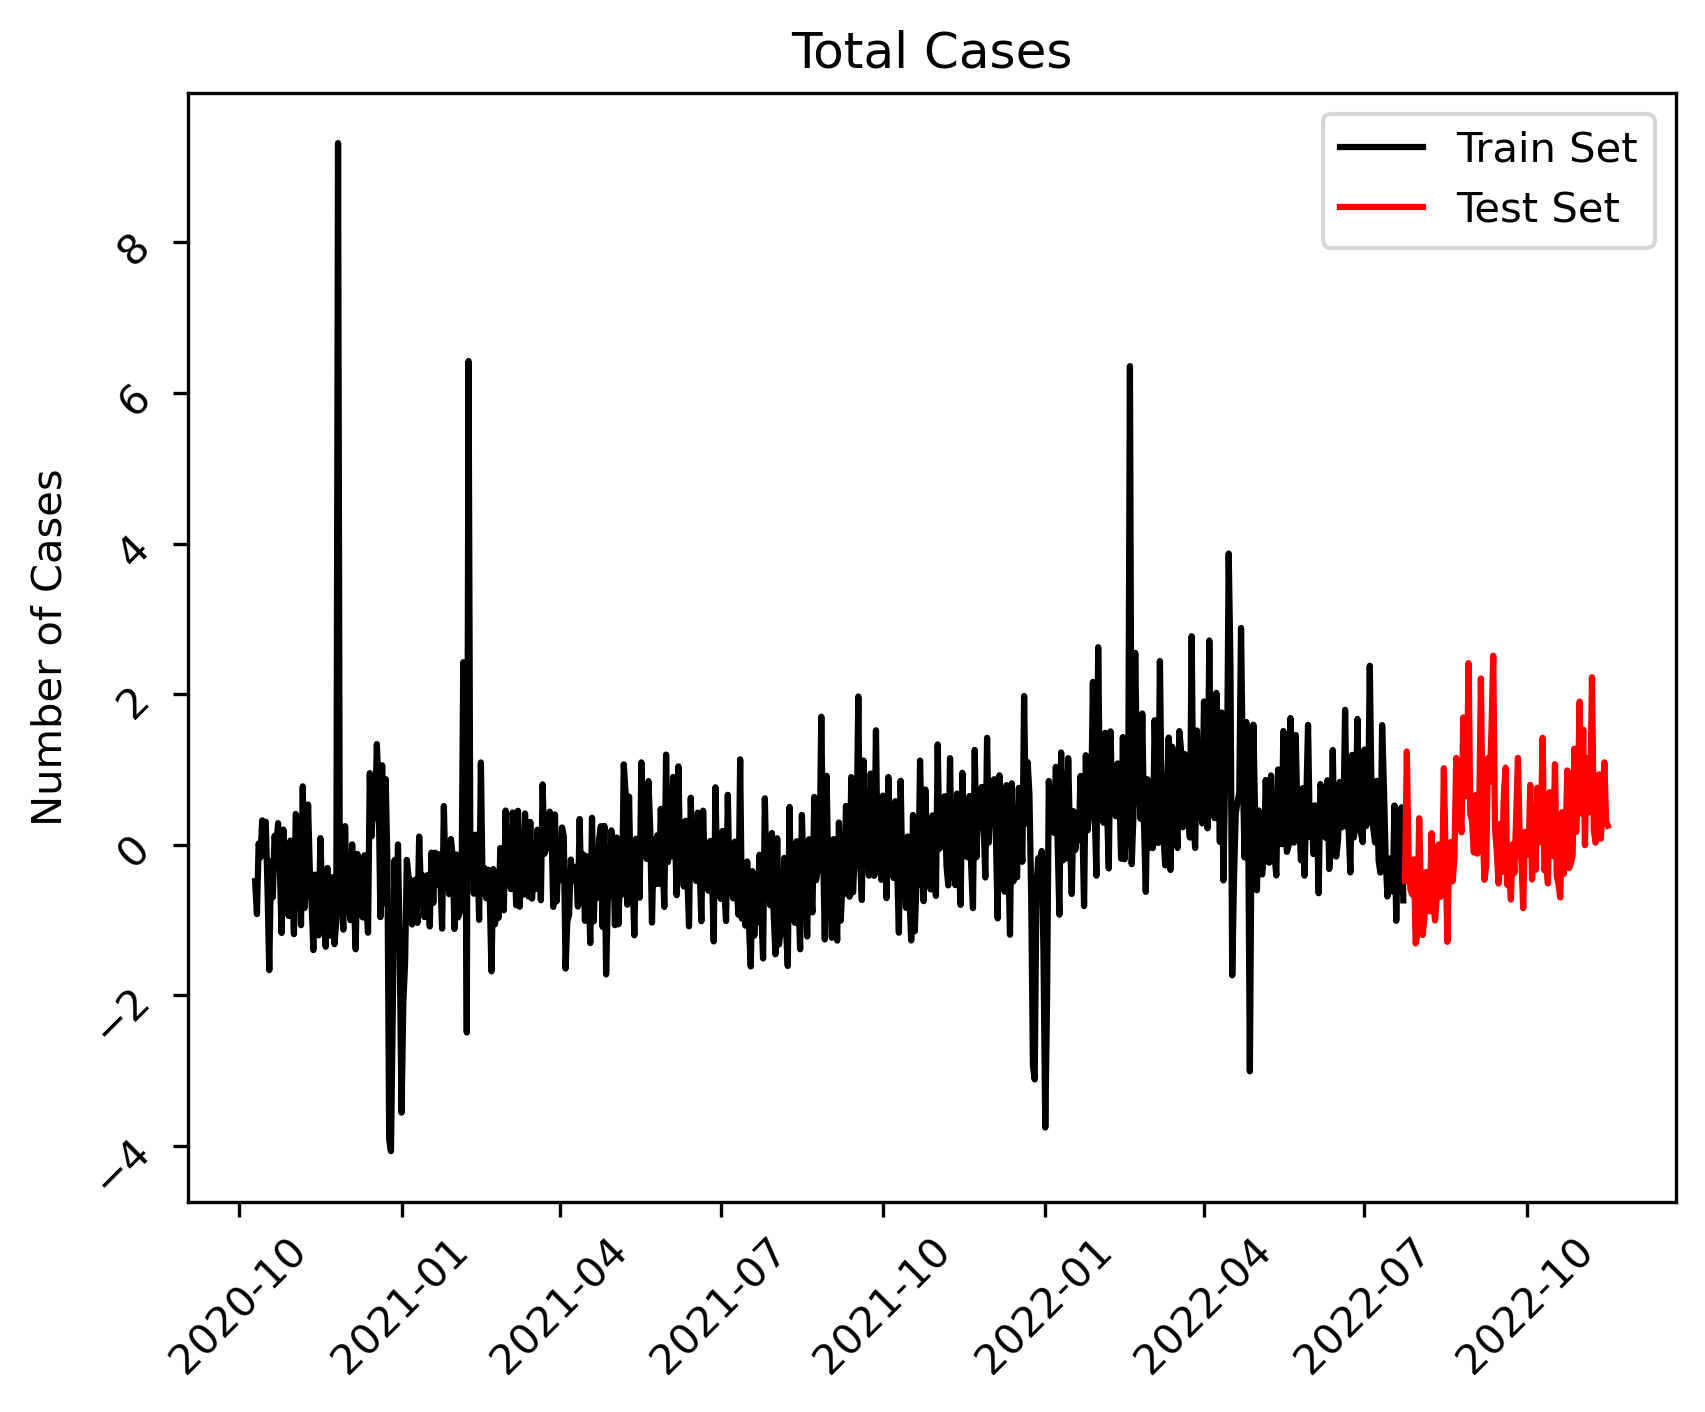
\includegraphics[width=\linewidth]{pics/cases_total_NL.png}
  \caption{The standardized total number of cases between the first of October 2020 and the first of October 2022}
  \label{fig:total cases NL}
\end{minipage}
\begin{minipage}{.5\textwidth}
  \centering
  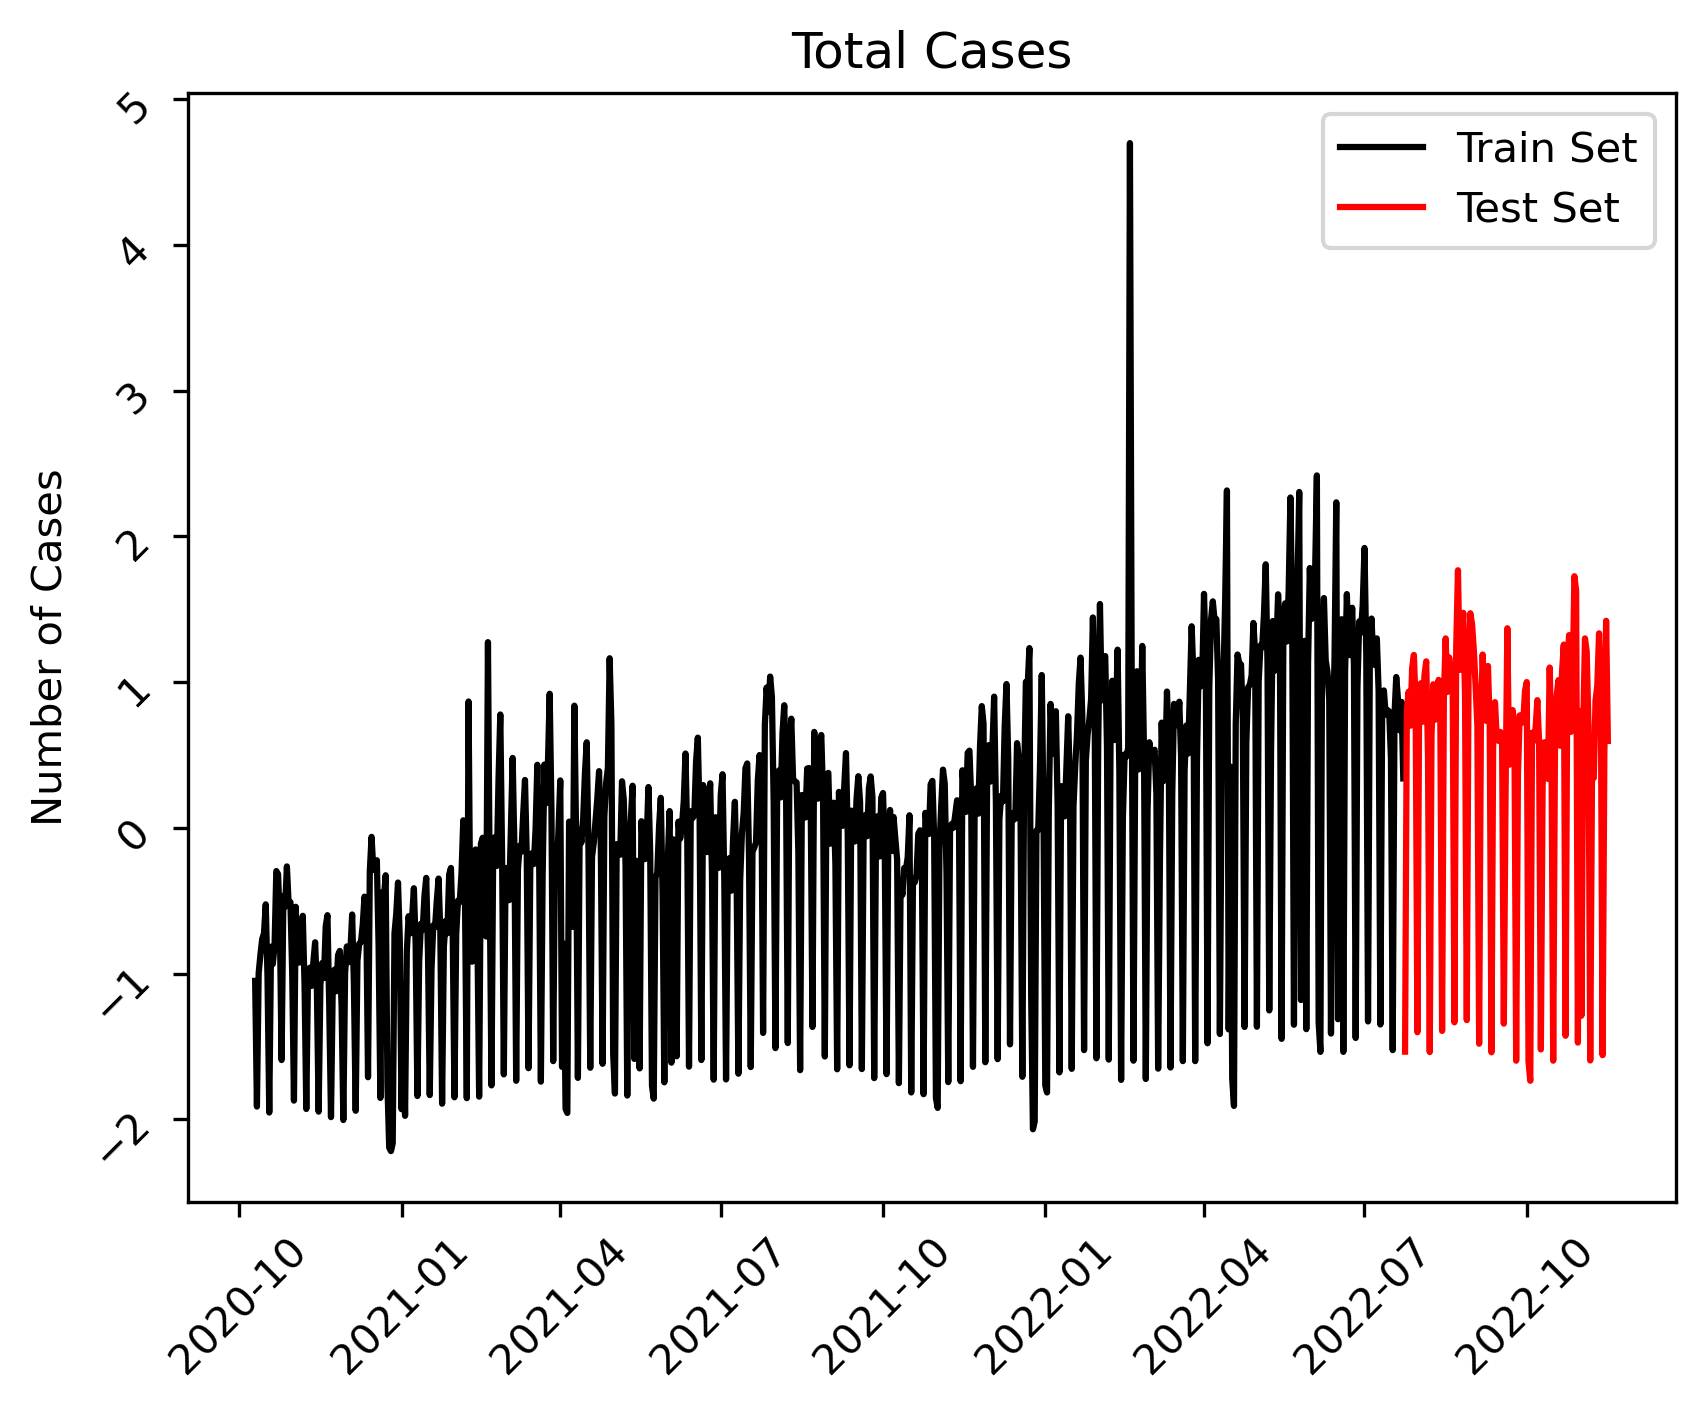
\includegraphics[width=\linewidth]{pics/cases_total_DE.png}
  \caption{The standardized total number of cases between the first of October 2020 and the first of October 2022}
  \label{fig:total cases DE}
\end{minipage}

\begin{minipage}{.5\textwidth}
  \centering
  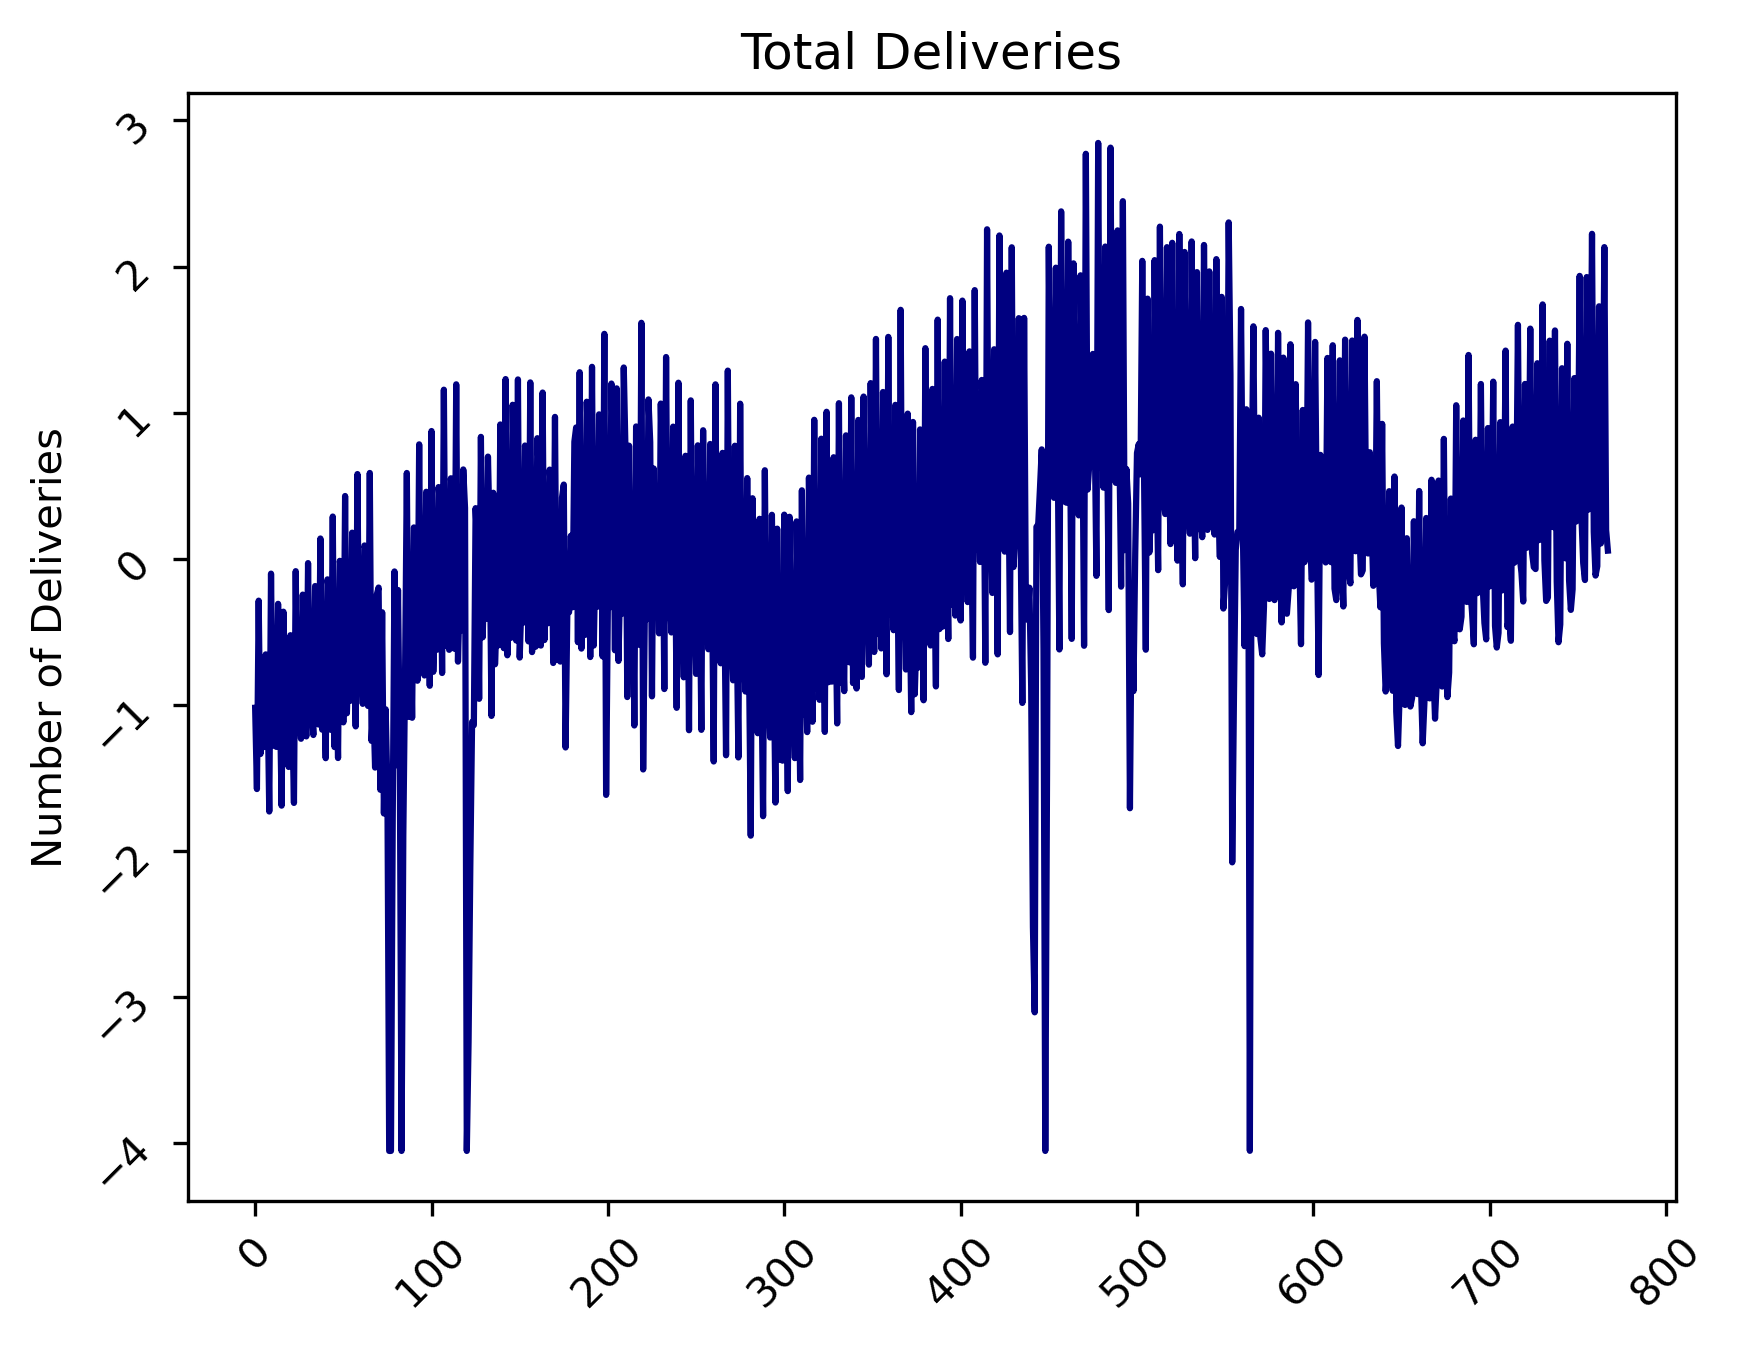
\includegraphics[width=\linewidth]{pics/deliveries_total_NL.png}
  \caption{The standardized total number of NL deliveries between the first of October 2020 and the first of October 2022}
  \label{fig:deliveries_NL}
\end{minipage}
\begin{minipage}{.5\textwidth}
  \centering
  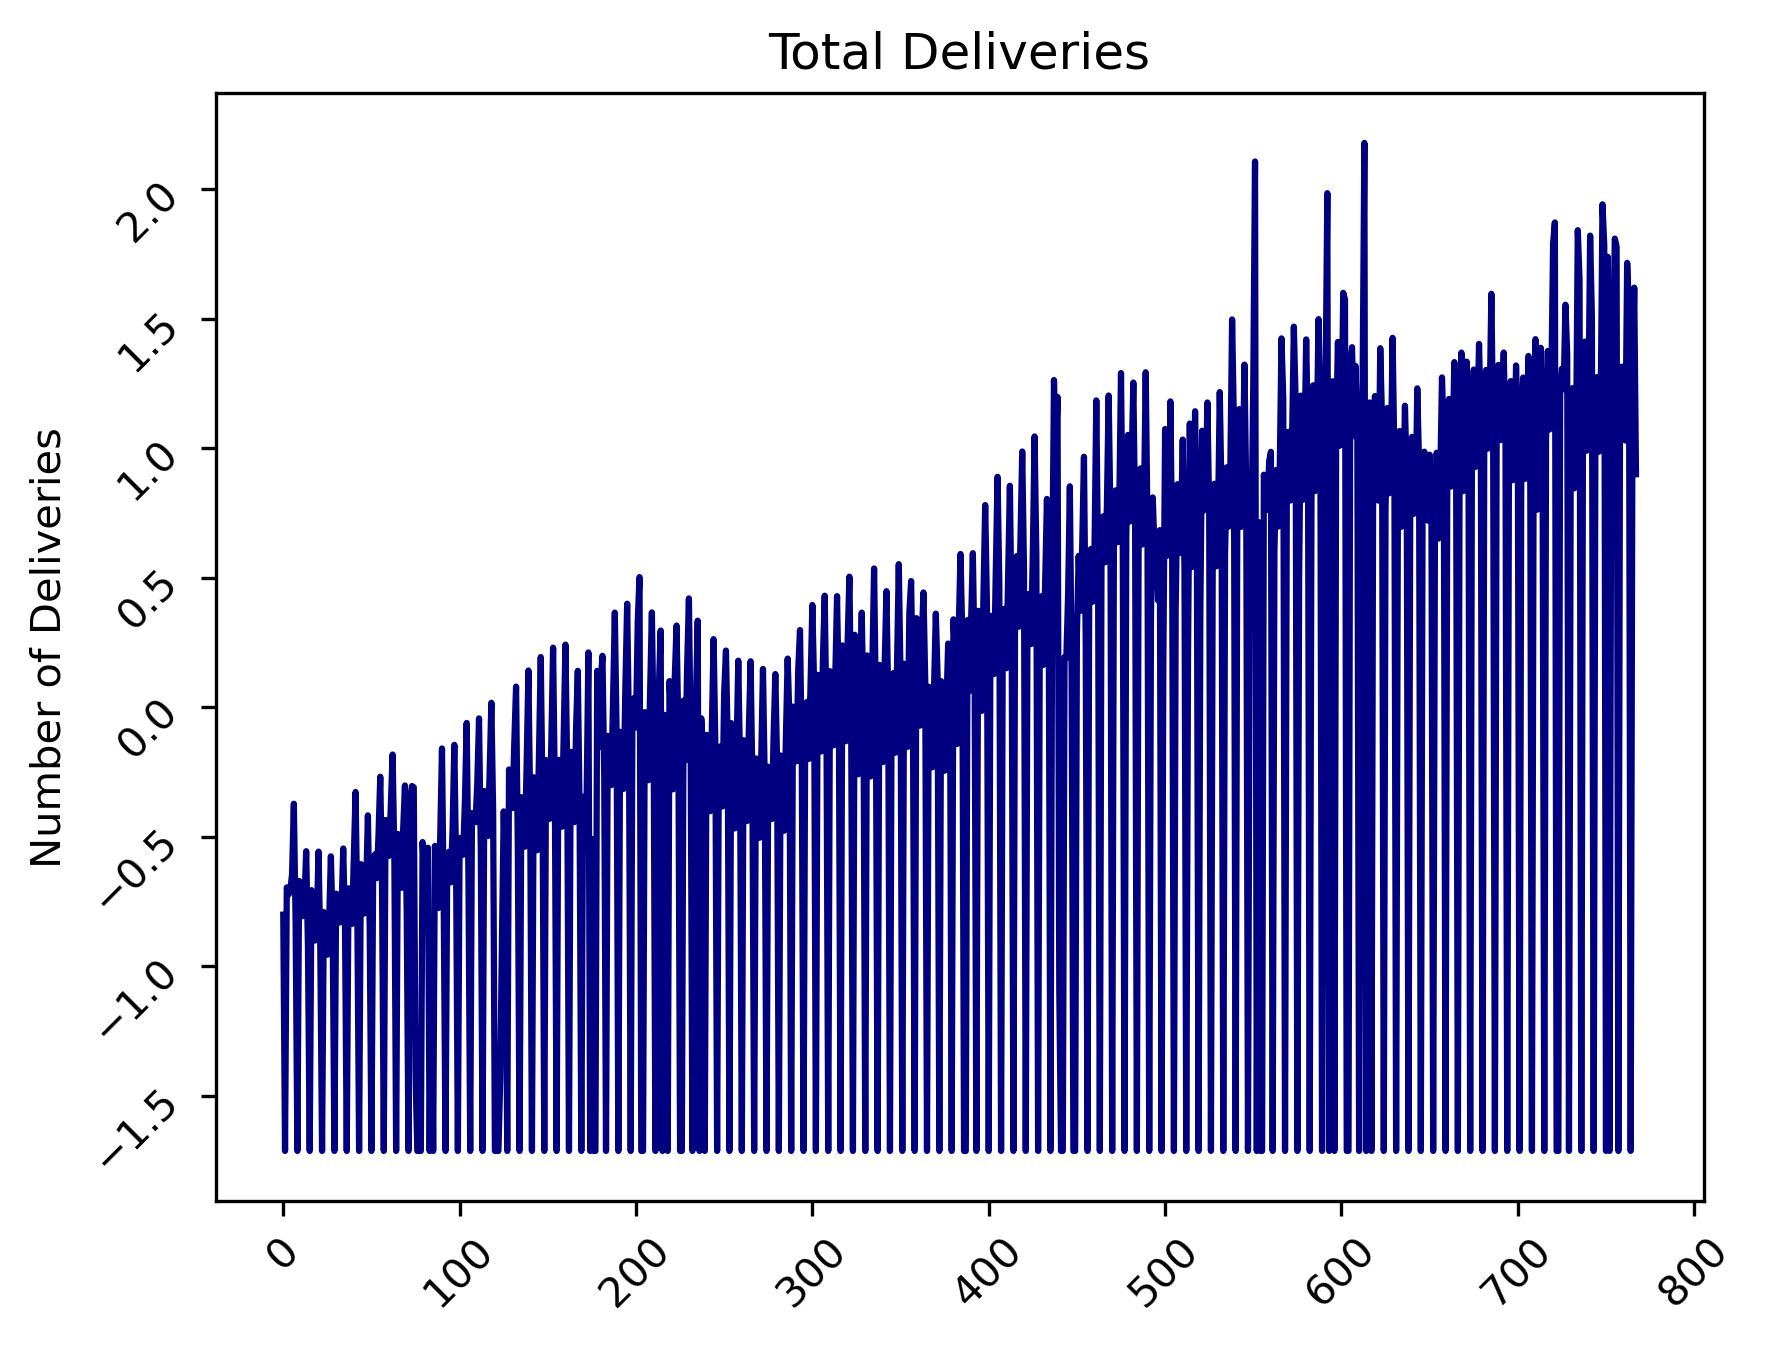
\includegraphics[width=\linewidth]{pics/deliveries_total_DE.png}
  \caption{The standardized total number of NL deliveries between the first of October 2020 and the first of October 2022}
  \label{fig:deliveries_DE}
\end{minipage}

\begin{minipage}{.5\textwidth}
  \centering
  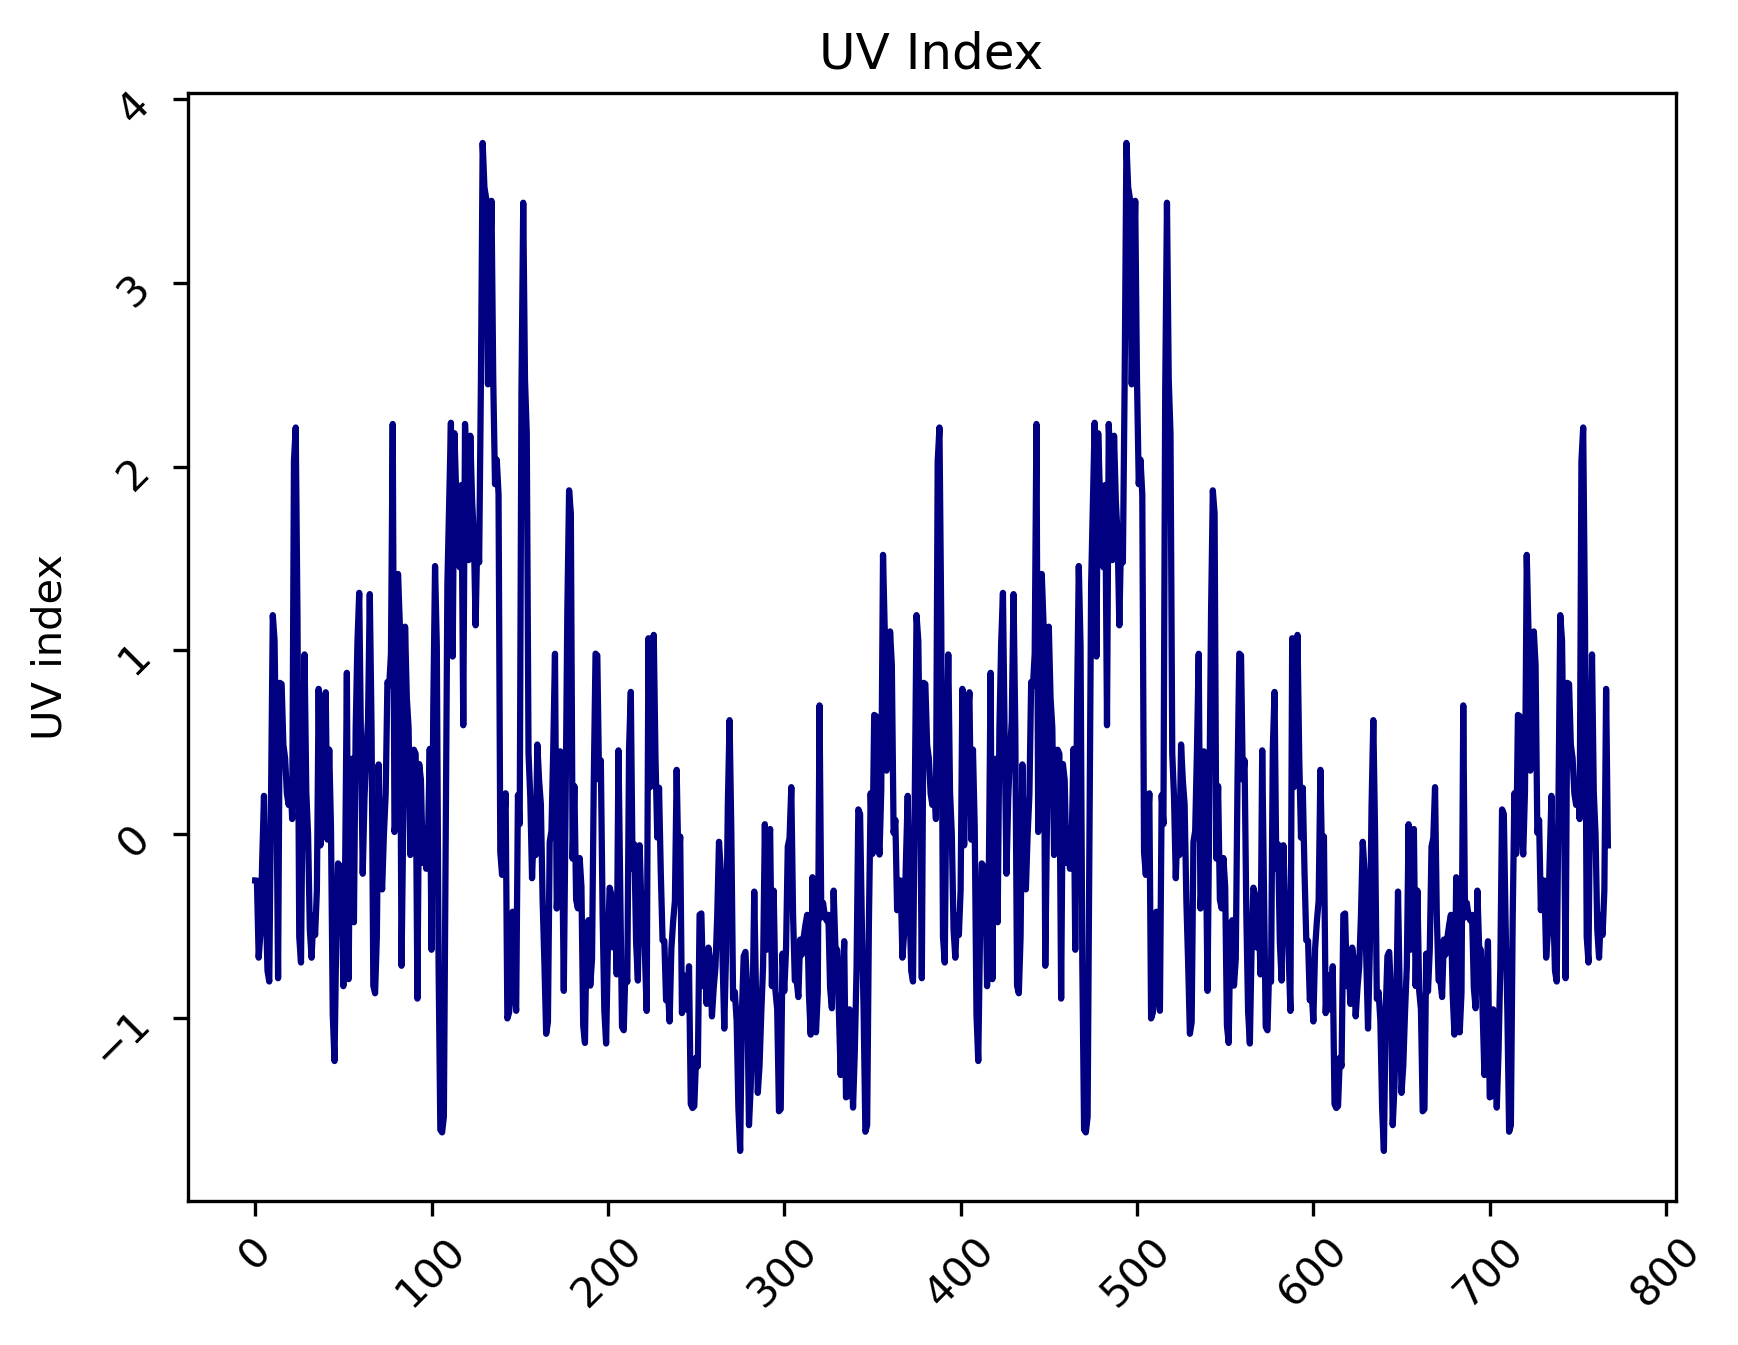
\includegraphics[width=\linewidth]{pics/uv_index_NL.png}
  \caption{The standardized UV index between the first of October 2020 and the first of October 2022}
  \label{fig:UV index NL}
\end{minipage}
\begin{minipage}{.5\textwidth}
  \centering
  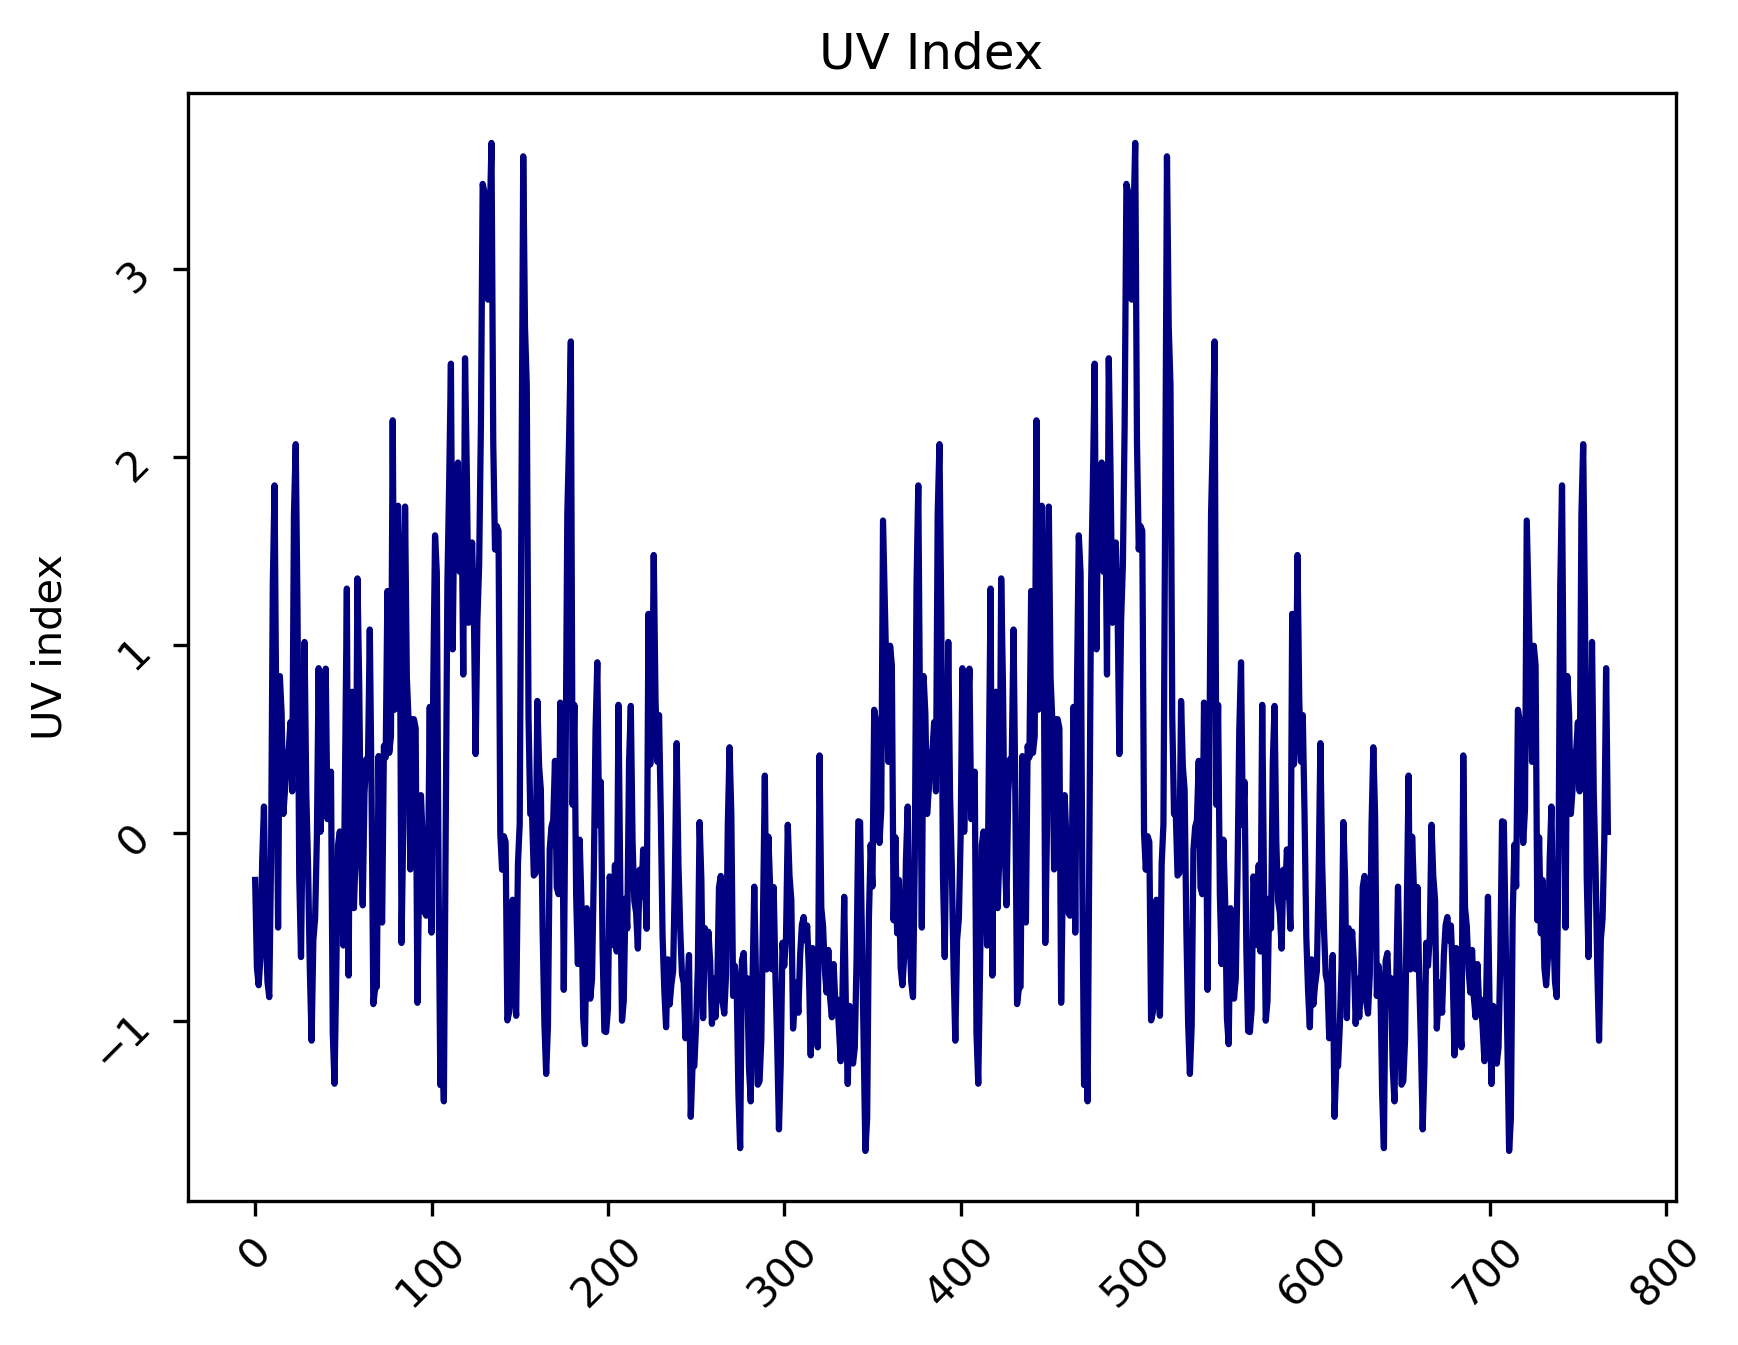
\includegraphics[width=\linewidth]{pics/uv_index_DE.png}
  \caption{The standardized UV index between the first of October 2020 and the first of October 2022}
  \label{fig:UV index DE}
\end{minipage}
\end{figure}

\begin{figure}
\begin{minipage}{.5\textwidth}
  \centering
  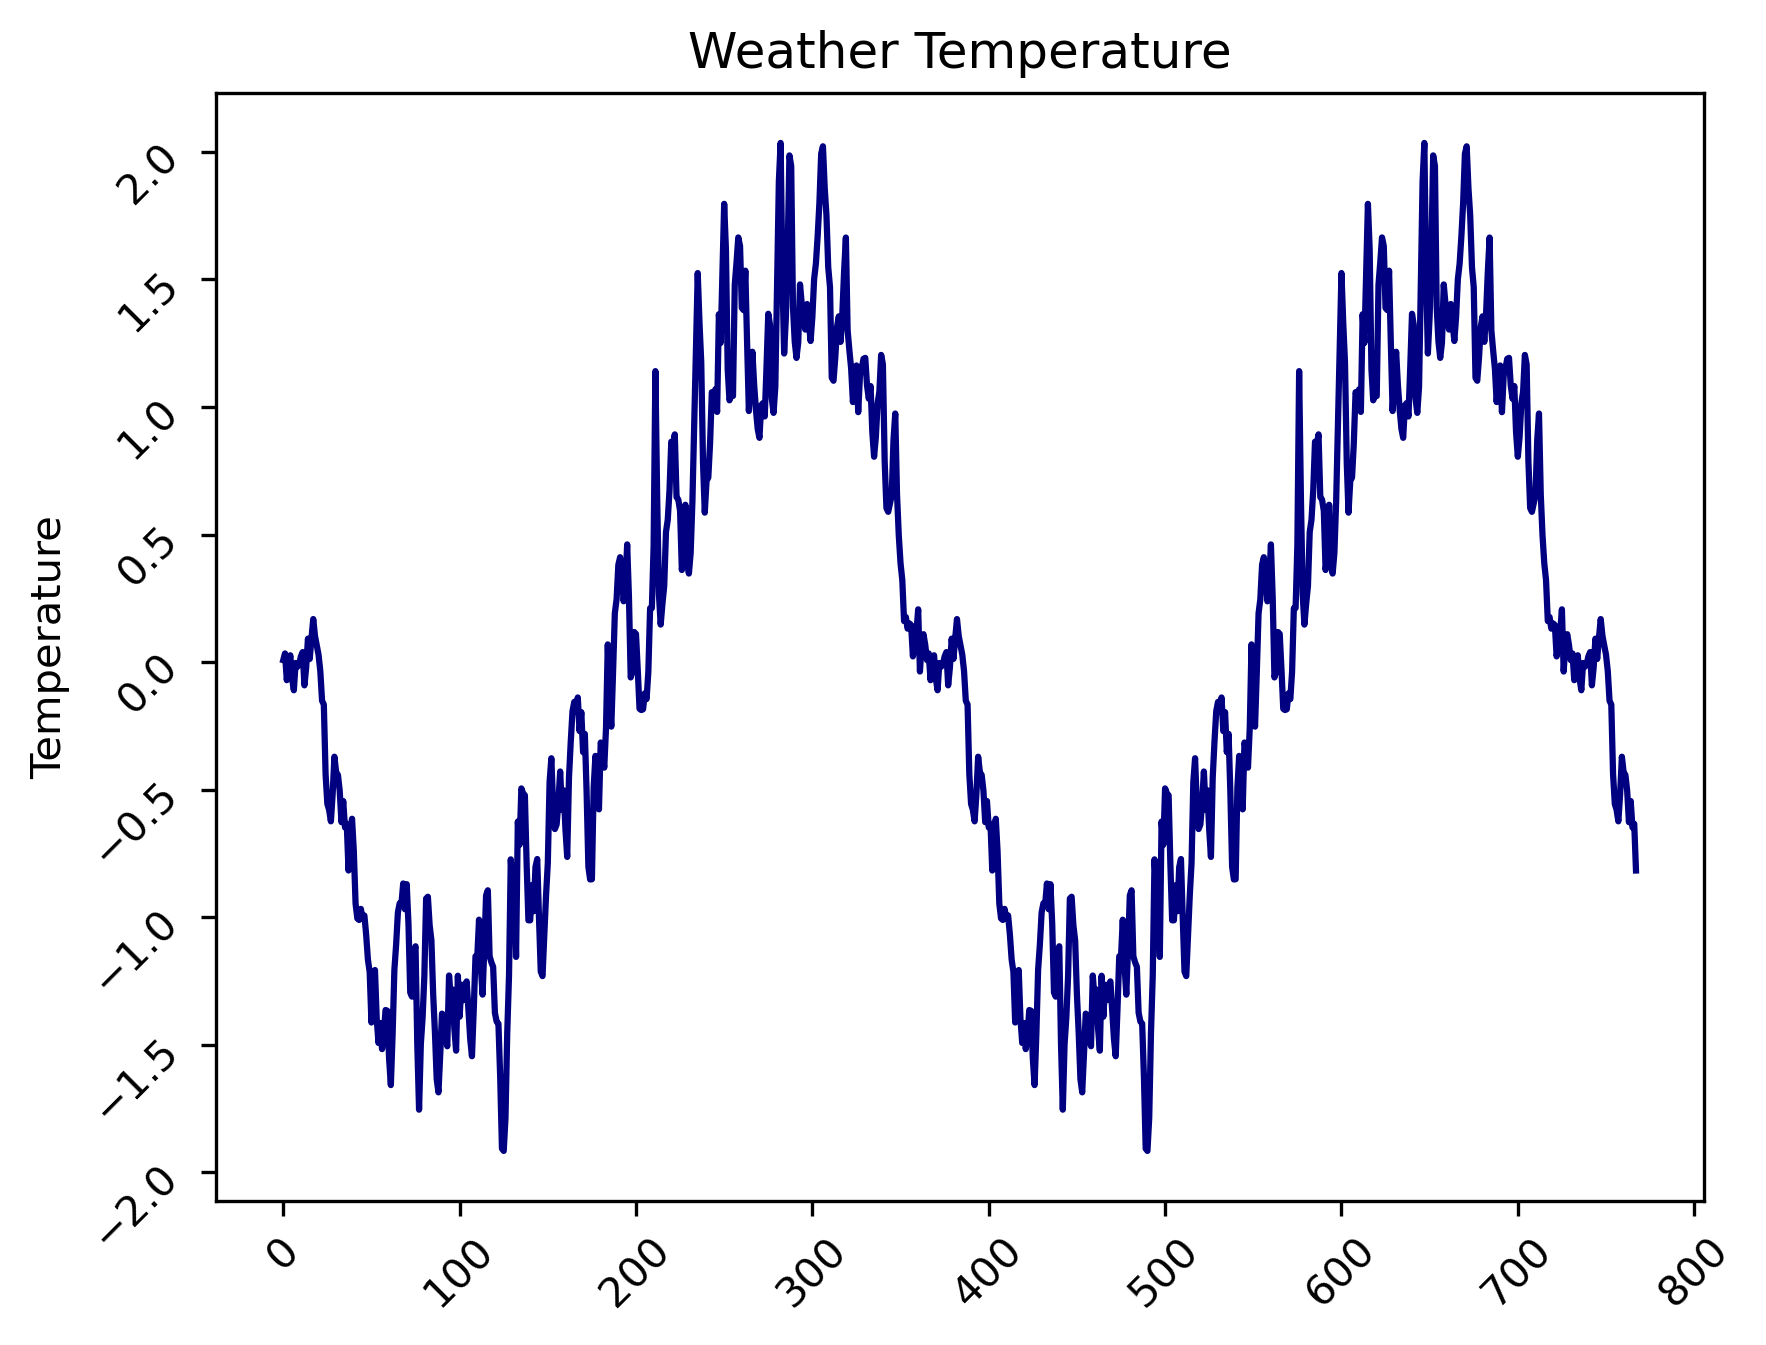
\includegraphics[width=\linewidth]{pics/temperature_total_NL.png}
  \caption{The standardized average temperature in NL between the first of October 2020 and the first of October 2022}
  \label{fig:temperature NL}
\end{minipage}
\begin{minipage}{.5\textwidth}
  \centering
  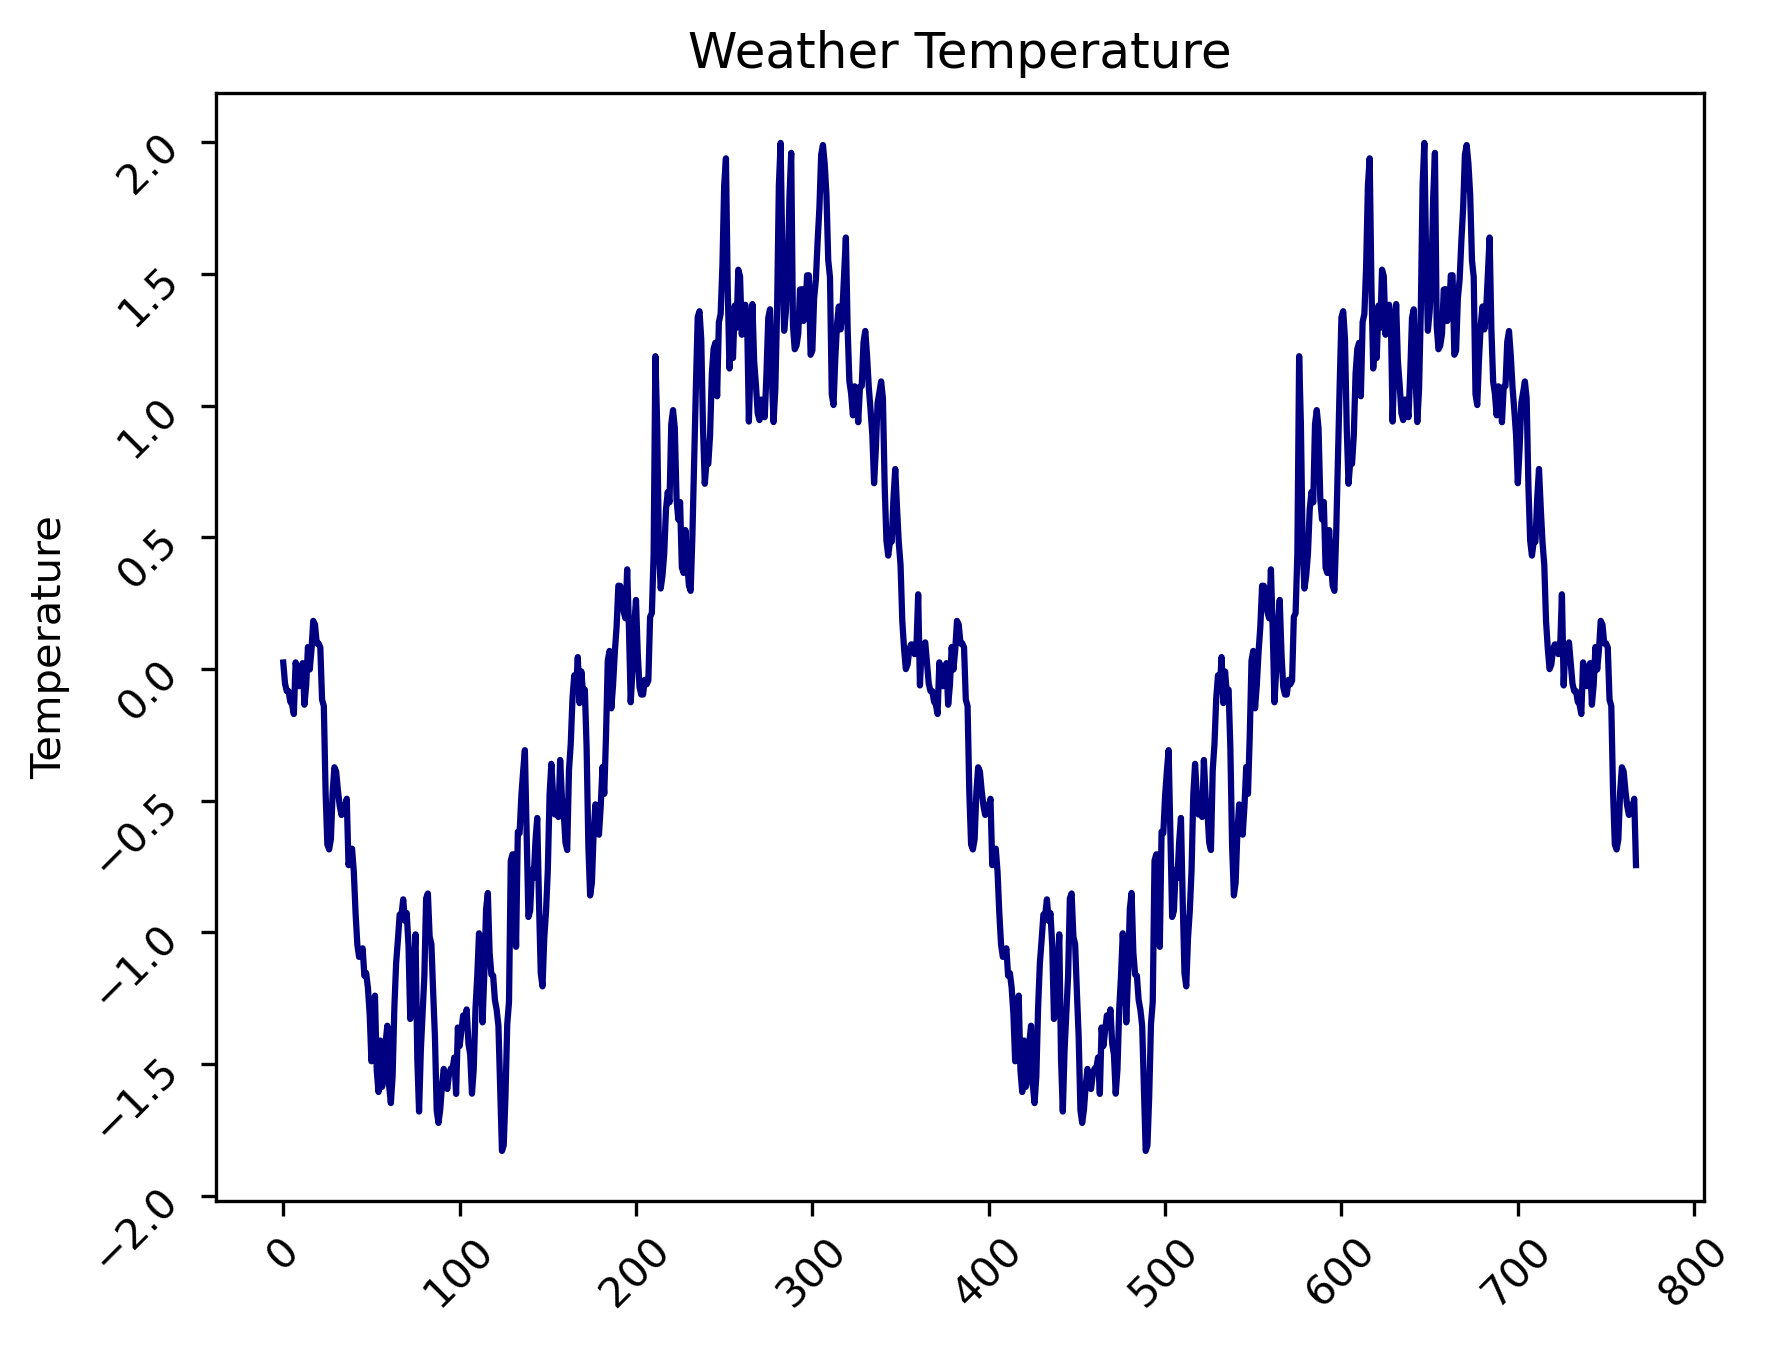
\includegraphics[width=\linewidth]{pics/temperature_total_DE.png}
  \caption{The standardized average temperature in NL between the first of October 2020 and the first of October 2022}
  \label{fig:temperature DE}
\end{minipage}
\end{figure}

As we can see in \autoref{tab:mean_var} the number of cases we want to predict has a high variance. This is expected as cases can come in at random. The high variance with incoming cases has been documented in previous literature \citep{Stolletz2011ArticleManagement}. The continuous numerical variables we want to use are described in \autoref{tab:coninuous_variables_mean_var}. The first feature, the daily number of deliveries is plotted in \autoref{fig:deliveries_NL} for the Netherlands and \autoref{fig:deliveries_DE} for Germany,  where you can a clear upward trend in Germany and a more seasonal trend in the Netherlands. You can also very clearly see the SUndays in Germany where there are no deliveries. The temperature is plotted in \autoref{fig:temperature NL} and in \autoref{fig:temperature DE} for Germany, in both coutries there is a similar seasonal effect where the temperature is lower in the winter and higher in the summer. The feature of the UV index is plotted in \autoref{fig:UV index NL} for the Netherlands and \autoref{fig:UV index DE} for Germany. The UV index graphs have a less clear seasonal effect than the temperature, but the effect does exist for both countries.\\

The choice of dependent variable as the number of cases (Total cases in \autoref{fig:total cases NL} for the Netherlands and in \autoref{fig:total cases DE} for Germany) instead of directly forecasting the workload has to do with a couple of reasons. The number of cases can be closed outside of the system which means the active time does not get recorded. If the workload gets very high, cases get closed in bulk. This means that agents will not spend any time on these cases. This is not a situation that should be taken into account in the data, because we want to predict the total number of cases that come in and should get attention from the agents if there are enough agnets. Another reason not to choose the workload as dependent variable is because there are always people optimising the operations at the customer success team. This means the workload per case can vary a lot and the historic data might not give a good indication on the workload per case in the future.\\

\subsection{Preprocessing}
Because the data is in different orders of magnitude, it is useful to standardize the data. This means that for all the models we will have:
\begin{equation}
    z = \frac{x - \hat{\mu}}{\hat{\sigma}}
\end{equation}
Where $\hat{\mu}$ is the sample mean of the data and $\hat{\sigma}$ is the sample standard deviation of the data. $\hat{\mu}$ and $\hat{\sigma}$ are saved such that it is possible to scale the data back in exactly the same way.\\

For the models, ARIMA, ARIMAX and VARIMAX models, it is important to take a look at order of integration I and for the lag selection it is important to look at the autocorrelation (Figures \ref{fig:autocorrelation NL} and \ref{fig:autocorrelation DE}) and the partial autocorrelation (Figures \ref{fig:partial autocorrelation NL} and \ref{fig:partial autocorrelation DE}). In \autoref{tab:dicktest} the p-values of the Engle-Granger cointegration test are displayed \citep{Engle1987Co-IntegrationTesting}. The Engle-Granger test has a null hypothesis of cointegration between Y and the first lag of Y. In \autoref{tab:dicktest} the p-values show that with a 5\% significance level we cannot say the data is not cointegrated if the order of differencing is 0 in both the Netherlands and Germany. If we difference the data 1 time, we can say with a significance level of less than 1\% that the data is not cointegrated. The same can be said if we difference the data two or three times. For the ARIMA models we will difference the data once since there is no advantage in continuing differencing if the data is not cointegrated and differencing the data has the disadvantage of becoming less easy to interpret and with every time the data is differenced, you lose 1 data point.\\
\begin{table}[]
    \centering
    \begin{tabular}{|c|c c|}\hline    
        Difference & Netherlands & Germany\\ \hline
        0 & 0.4905  & 0.0921 \\
        1 & 0.0 & 0.0 \\
        2 & 0.0 & 0.0 \\
        3 & 0.0 & 0.0 \\
        4 & 0.0 & 0.0 \\
    \hline 
    \end{tabular}
    \caption{P-values of the augmented Dickey Fuller test for stationarity on total number of cases}
    \label{tab:dicktest}
\end{table}

\begin{figure}
\begin{minipage}{.5\textwidth}
    \centering
    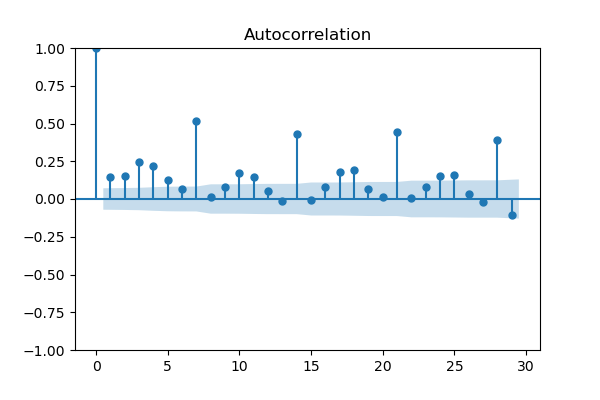
\includegraphics[width=\linewidth]{pics/acf_1_diff_NL.png}
    \caption{Autocorrelation plot of first differenced data in the Netherlands}
    \label{fig:autocorrelation NL}
\end{minipage}
\begin{minipage}{.5\textwidth} 
    \centering
    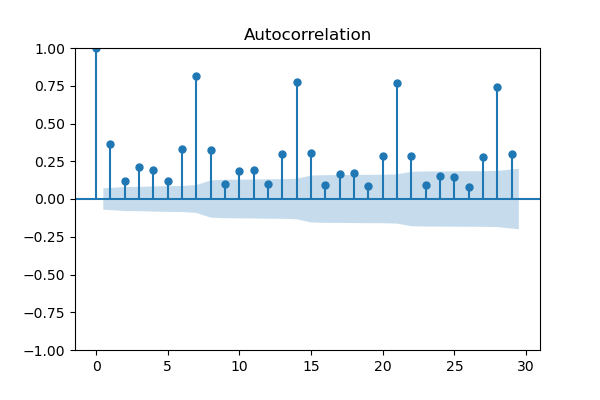
\includegraphics[width=\linewidth]{pics/acf_1_diff_DE.png}
    \caption{Autocorrelation plot of first differenced data in Germany}
    \label{fig:autocorrelation DE}
\end{minipage}
\end{figure}
\begin{figure}
\begin{minipage}{.5\textwidth}
    \centering
    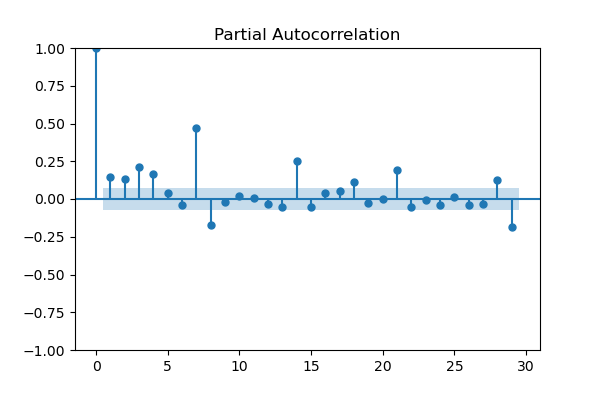
\includegraphics[width=\linewidth]{pics/pacf_1_diff_NL.png}
    \caption{Partial Autocorrelation plot of first differenced data in the Netherlands}
    \label{fig:partial autocorrelation NL}
\end{minipage}
\begin{minipage}{.5\textwidth} 
    \centering
    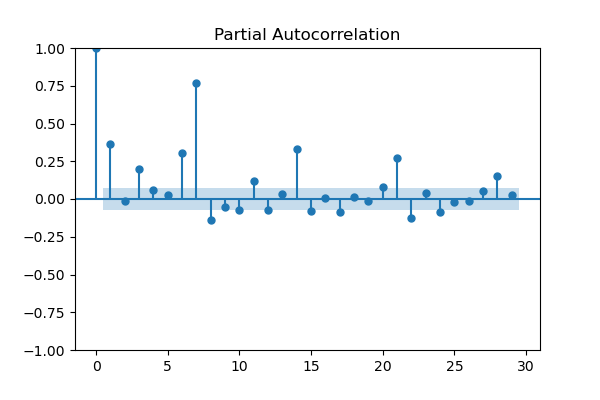
\includegraphics[width=\linewidth]{pics/pacf_1_diff_DE.png}
    \caption{Partial autocorrelation plot of first differenced data in Germany}
    \label{fig:partial autocorrelation DE}
\end{minipage}
\end{figure}
\section{Results}
\label{seq:results}
In this section, the fitted parameters of the parametric models will be reported, as well as the performance of each model.
\subsection{Model Estimation}
\label{subseq:model estimation}
All the models are estimated to fit the data. In this section there are many parameters which need to be described. The parameters all have their own notation. This means that in the following graphs the following means: $\sigma_{\eta}^2$ is the parameter corresponding to the variance of the state vector, $\sigma_{\epsilon}^2$ is the parameter corresponding to the estimated variance of the error terms, $\beta_1$ corresponds to the first lag of the data, $\beta_7$ corresponds to the seventh lag of the data, $\gamma_1$ corresponds to the weather temperature data, $\gamma_2$ corresponds is the UV index data, $\gamma_3$ corresponds to the number of deliveries, $\gamma_4$ corresponds to the number of regions with vacation, $\gamma_5$ corresponds to 1 if there is a national holiday, 0 otherwise, $\gamma_{6-12}$  are constants for the day of the week and $\theta_0$ is the moving average component.\\

\begin{table}[]
    \centering
    \begin{tabular}{|c|c c c||c|c c c|}\hline
        NL & coefficient & t-statistic & p-value & DE & coefficient & t-statistic & p-value\\\hline        
        $\sigma_{\epsilon}$ & 0.429 & 10.984 & 0.0 & $\sigma_{\epsilon}$ & 0.349 & 8.943 & 0.0\\
        $\sigma_{\eta}$ & 0.002 & 0.044 & 0.965 & $\sigma_{\eta}$ & 0.001 & 0.015 & 0.988\\\hline
    \end{tabular}
    \caption{Local Level Model regression results with the coefficient, t-statistic and p-values for the Dutch and German estimation}
    \label{tab:local_level_regression_Results}
\end{table}
The most basic model is the local level model with two estimated values of $\sigma$. The estimated parameters of this model can be found in \autoref{tab:local_level_regression_Results}. The value of $\sigma_{\epsilon}$ is quite large and therefore also significant for both the Dutch and the German data with a p-value smaller than 0.0005. This makes a very low signal to noise ratio of 0.0047 for the Netherlands and 0.0029 for Germany. That means there is there is a lot of noise in the data which is expected as cases at customer service can come with a very high variance. The estimated values of $\sigma_{\eta}$  is in both cases much smaller and definitely not significant.\\

\begin{table}[]
    \centering
    \begin{tabular}{|c|c c c||c|c c c|}\hline
        NL & coefficient & t-statistic & p-value & DE & coefficient & t-statistic & p-value\\\hline     
        $\sigma_{\epsilon}$ & 0.236 & 6.046 & 0.0 & $\sigma_{\epsilon}$ & 0.031 & 0.791 & 0.429\\
        $\sigma_{\eta}$ & 0.001 & 0.013 & 0.99 & $\sigma_{\eta}$ & 0.002 & 0.05 & 0.96\\
        $\gamma_{1}$ & 0.033 & 0.828 & 0.408 & $\gamma_{1}$ & 0.068 & 1.686 & 0.092\\
        $\gamma_{2}$ & 0.048 & 1.231 & 0.219 & $\gamma_{2}$ & 0.035 & 0.887 & 0.375\\
        $\gamma_{3}$ & 0.268 & 8.194 & 0.0 & $\gamma_{3}$ & 0.856 & 25.361 & 0.0\\
        $\gamma_{4}$ & -0.15 & -3.935 & 0.0 & $\gamma_{4}$ & -0.015 & -0.413 & 0.68\\
        $\gamma_{5}$ & -0.163 & -4.37 & 0.0 & $\gamma_{5}$ & -0.038 & -0.957 & 0.339\\
        $\gamma_{6}$ & 0.557 & 15.406 & 0.0 & $\gamma_{6}$ & 0.306 & 8.883 & 0.0\\
        $\gamma_{7}$ & 0.284 & 8.299 & 0.0 & $\gamma_{7}$ & 0.34 & 10.032 & 0.0\\
        $\gamma_{8}$ & 0.349 & 9.812 & 0.0 & $\gamma_{8}$ & 0.369 & 10.401 & 0.0\\
        $\gamma_{9}$ & 0.298 & 7.631 & 0.0 & $\gamma_{9}$ & 0.365 & 9.439 & 0.0\\
        $\gamma_{10}$ & 0.489 & 15.576 & 0.0 & $\gamma_{10}$ & 0.359 & 11.397 & 0.0\\
        $\gamma_{11}$ & 0.306 & 8.935 & 0.0 & $\gamma_{11}$ & 0.307 & 9.586 & 0.0\\
        $\gamma_{12}$ & 0.16 & 4.737 & 0.0 & $\gamma_{12}$ & 0.245 & 7.53 & 0.0\\\hline
    \end{tabular}
    \caption{Regression model results with the coefficient, t-statistic and p-values for the Dutch and German estimation}
    \label{tab:regression_model_results}
\end{table}
The expansion of the local level model to the regression model with parameters to the regression model described in \autoref{tab:regression_model_results}. The regression model only has a significant $\sigma_{\epsilon}$ in the Dutch data. The German data has no significant $\sigma_\epsilon$. This is probably because the German data has more steep differences in the data which can be explained better by other factors like the day of the week. Just as with the local level model, the $\sigma_\eta$ is in both countries not significant. Something to note is that the weather data ($\gamma_1$ and $\gamma_2$) are not significant in the Netherlands with parameters of only 0.268 and -0.15, but the temperature ($\gamma_2$) in Germany is significant at the 10\% significance interval with a coefficient of 0.375. The number of deliveries ($\gamma_3$) is significant in both the Netherlands and Germany and it is worth it to take a look at how large the difference is between the Netherlands (0.268) and Germany (0.856) in Number of deliveries coefficient pointing to a more reliable cases per delivery relationship in Germany. The coefficients corresponding to vacations ($\gamma_4$) and holidays ($\gamma_5$) are significant in the Netherlands and not in Germany. This could be because the German operations have more days where the Customer Service is offline and there are no deliveries. In the Netherlands this only happens at holidays, but in Germany this happens also at Sundays. The last thing to point out is that all the constants for the different days ($\gamma_6$-$\gamma_{12}$) are significant, pointing to a strong relation between what day it is and how many cases come in.\\

\begin{table}[]
    \centering
    \begin{tabular}{|c|c c c||c|c c c|}\hline
        NL & Coefficient & t-statistic & p-value & DE & Coefficient & t-statistic & p-value\\\hline
        $\beta_1$ & 0.154 & 3.867 & 0.0 & $\beta_1$ & 0.177 & 4.594 & 0.0\\
        $\beta_7$ & 0.500 & 12.598 & 0.0 & $\beta_7$ & 0.814 & 21.104 & 0.0\\
        $\theta_0$ & -0.043 & -1.112 & 0.267 & $\theta_0$ & -0.045 & -1.147 & 0.252\\\hline
    \end{tabular}
    \caption{ARIMA regression results with the coefficient, t-statistic and p-values for the Dutch and German estimation}
    \label{tab:ARIMA_estimation_results}
\end{table}
In the results of the ARIMA regression are given in in \autoref{tab:ARIMA_estimation_results}. It is remarkable that the moving average components are not significant for both countries. Also note that the seventh lag ($\beta_7$) has a higher coefficient than the first lag, pointing to a strong weekly relationship.\\

\begin{table}[]
    \centering
    \begin{tabular}{|c|c c c||c|c c c|}\hline
        NL & Coefficient & t-statistic & p-value & DE & Coefficient & t-statistic & p-value\\\hline
        $\gamma_{1}$ & 0.04 & 1.011 & 0.312 & $\gamma_{1}$ & 0.086 & 2.17 & 0.03\\
        $\gamma_{2}$ & 0.04 & 0.997 & 0.319 & $\gamma_{2}$ & 0.052 & 1.293 & 0.196\\
        $\gamma_{3}$ & 0.334 & 8.372 & 0.0 & $\gamma_{3}$ & 0.800 & 22.371 & 0.0\\
        $\gamma_{4}$ & -0.089 & -2.301 & 0.022 & $\gamma_{4}$ & 0.002 & 0.047 & 0.963\\
        $\gamma_{5}$ & -0.128 & -3.006 & 0.003 & $\gamma_{5}$ & -0.041 & -0.977 & 0.329\\
        $\gamma_{6}$ & 0.151 & 3.857 & 0.0 & $\gamma_{6}$ & 0.174 & 4.434 & 0.0\\
        $\gamma_{7}$ & -0.155 & -3.948 & 0.0 & $\gamma_{7}$ & 0.098 & 2.503 & 0.013\\
        $\gamma_{8}$ & -0.022 & -0.565 & 0.572 & $\gamma_{8}$ & 0.106 & 2.703 & 0.007\\
        $\gamma_{9}$ & -0.077 & -1.964 & 0.05 & $\gamma_{9}$ & 0.106 & 2.725 & 0.007\\
        $\gamma_{10}$ & 0.06 & 1.547 & 0.122 & $\gamma_{10}$ & 0.097 & 2.483 & 0.013\\
        $\gamma_{11}$ & -0.139 & -3.566 & 0.0 & $\gamma_{11}$ & 0.033 & 0.849 & 0.396\\
        $\gamma_{12}$ & -0.176 & -4.517 & 0.0 & $\gamma_{12}$ & 0.005 & 0.14 & 0.889\\
        $\beta_{1}$ & 0.206 & 5.176 & 0.0 &$\beta_{1}$ & 0.186 & 4.823 & 0.0\\
        $\beta_{7}$ & 0.131 & 3.287 & 0.001 & $\beta_{7}$ & 0.063 & 1.628 & 0.104\\
        $\theta_{0}$ & 0.049 & 1.281 & 0.201 & $\theta_0$ & 0.229 & 21.508 & 0.0\\\hline
    \end{tabular}
    \caption{ARIMAX regression results with the coefficient, t-statistic and p-values for the Dutch and German estimation}
    \label{tab:arimax_estimation}
\end{table}
The estimated parameters of the ARIMAX regression are given in \autoref{tab:arimax_estimation} and tell us more about the interaction between the explanatory variables and the lags. Just as in the regression model, the weather data only has a significant effect on the German cases and from the two weather variables, only the temperature ($\gamma_1$) has a significant effect with a coefficient of 0.086. Also as in the regression model, the number of deliveries ($\gamma_3$) has a strong effect on both data sets, but it has an even larger effect in the German data with coefficients of 0.800 in Germany against only 0.344. Things start to become different looking at the national holidays ($\gamma_6$) which is significant in the ARIMAX model for Germany, but not in the regression model. The coefficient corresponding to the national holidays is 0.151 in the Netherlands and 0.174 in Germany which is a large difference with the regression model. Another important difference between the ARIMAX model and the regression model is that the daily constants have a very different level of significance. The regressors are smaller and multiple daily constants have no significance at the 5\% significance level. A remarkable result is the non significance of the Sunday constant $\lambda_{12}$ in Germany which has has coefficient of only 0.063. The German Sunday drop in cases is not explained as a drop in cases on Sunday by the ARIMAX model, but with the drop in deliveries at Sundays. You can also see a difference with the ARIMA as we see the seventh lag drop in importance and in the German data, the seventh lag is not even significant at the 10\% significance level. Another difference with the ARIMA model is that the German data has a significant moving average component with a coefficient of 0.229 comparing to the Dutch moving average component of 0.049.\\

\begin{table}[]
    \centering
    \begin{tabular}{|c|c c c||c|c c c|}\hline
        NL & Coefficient & t-statistic & p-value & DE & Coefficient & t-statistic & p-value\\\hline
        $\gamma_{1}$ & 0.041 & 1.076 & 0.282 & $\gamma_{1}$ & 0.084 & 2.157 & 0.031\\
        $\gamma_{2}$ & 0.041 & 1.096 & 0.273 & $\gamma_{2}$ & 0.052 & 1.27 & 0.205\\
        $\gamma_{3}$ & 0.338 & 9.636 & 0.0 & $\gamma_{3}$ & 0.795 & 20.94 & 0.0\\
        $\gamma_{4}$ & -0.089 & -2.509 & 0.012 & $\gamma_{4}$ & 0.001 & 0.028 & 0.978\\
        $\gamma_{5}$ & -0.125 & -3.518 & 0.0 & $\gamma_{5}$ & -0.041 & -1.045 & 0.296\\
        $\gamma_{6}$ & 0.22 & 6.54 & 0.0 & $\gamma_{6}$ & 0.066 & 1.96 & 0.05\\
        $\gamma_{7}$ & -0.075 & -2.357 & 0.019 & $\gamma_{7}$ & -0.0 & -0.0 & 1.0\\
        $\gamma_{8}$ & 0.05 & 1.493 & 0.136 & $\gamma_{8}$ & 0.006 & 0.182 & 0.856\\
        $\gamma_{9}$ & 0.0 & 0.0 & 1.0 & $\gamma_{9}$ & 0.006 & 0.153 & 0.879\\
        $\gamma_{10}$ & 0.131 & 4.184 & 0.0 & $\gamma_{10}$ & -0.002 & -0.049 & 0.961\\
        $\gamma_{11}$ & -0.062 & -1.908 & 0.057 & $\gamma_{11}$ & -0.063 & -2.022 & 0.044\\
        $\gamma_{12}$ & -0.098 & -3.117 & 0.002 & $\gamma_{12}$ & -0.085 & -2.73 & 0.007\\
        $\beta_{1}$ & 0.199 & 6.267 & 0.0 & $\beta_{1}$ & 0.174 & 5.803 & 0.0\\
        $\beta_{7}$ & 0.133 & 4.365 & 0.0 & $\beta_{7}$ & 0.078 & 2.587 & 0.01\\
        $\lambda^{(1)}$ & -0.846 & -0.0 & 1.0 & $\lambda^{(1)}$ & -0.811 & -0.0 & 1.0\\
        $\lambda^{(2)}$ & -0.104 & -0.0 & 1.0 & $\lambda^{(2)}$ & -0.104 & -0.0 & 1.0\\ \hline
    \end{tabular}
    \caption{Fused lasso regression results with the coefficient, t-statistic and p-values for the Dutch and German estimation}
    \label{tab:FLASSO_estimation_results}
\end{table}
The fused lasso seems to behave in a way that is very similar to the ARIMAX. This is not really surprising as the regression results given in \autoref{tab:FLASSO_estimation_results} show two insignificant values of $\lambda$, and the values of $\theta_0$ in the ARIMAX model are also insignificant (\autoref{tab:arimax_estimation}). The expectation would be that the coefficients are very close to the ARIMAX coefficients. The exception to this are the day of the week constants. So in line with this it seems like the regressions of the ARIMA and the LASSO are not very much different for the Dutch data which is supported by the Diebold Mariano tests. The regressions however are different from each other with the German data as it has larger coefficients for the weekday variables which are different with the two models.\\


\subsection{Forecast results}
\label{subsec:forecast_results}
The performance of the forecasts are measured on the similarity to the test set. There are tests performed on three horizons of forecasts: 7 days (\autoref{tab:1 week ahead}), 28 days (\autoref{tab:4 weeks ahead}) and 49 days (\autoref{tab:7 weeks ahead}). For all the models the MAE (Mean Absolute Error), MSE (Mean Squared Error), RMSE (root Mean Squared Error) and MAPE (Mean Absolute Percentage Error) are calculated. We see that all of the models perform better on the Dutch data. This can be expected because the Dutch operations are going on for a longer and are more mature while the German operations are newer and less mature. The p-values of the Diebold Mariano test can be seen in Tables \ref{tab:1 week ahead diebold}, \ref{tab:4 week ahead dm} and \ref{tab:7 weeks ahead dm} for the 1 week, 4 weeks and 7 weeks horizons.\\

The better performance in the Netherlands can have multiple reasons. The Germans have done good work improving the picking process at the fulfillment centers and streamlining customer communication. This however means that the models cannot yet learn from these improvements as they are continuously implemented. The hope is that as the German market matures the models in the future will improve their performance.\\

\begin{table}[]
    \centering
    \begin{tabular}{|c|c c c|}\hline
        Netherlands & MAE & RMSE & MAPE\\\hline
        Local Level Model & 384.729  & 496.16 & 0.114\\
        Regression Model & 299.849 & 385.391 & 0.087\\
        ARIMA & 286.902 & 412.48 & 0.078\\
        ARIMAX & 242.294 & 322.536 & 0.068\\
        VARIMAX & 250.475 & 325.205 & 0.071\\
        Fused Lasso & 240.894 & 321.319 & 0.068\\
        XGBoost & 308.925 & 418.073 & 0.088\\
        Neural Network & 291.157 & 365.504 & 0.083\\
        Multivariate Neural Network & 311.359 & 390.876 & 0.09\\
        Mixed Model & 266.868 & 342.778 & 0.076\\\hline\hline
        Germany & MAE & RMSE & MAPE\\\hline
        Local Level Model & 435.601 & 631.483 & 0.223\\
        Regression Model & 198.15 & 237.948 & 0.238\\
        ARIMA & 261.571 & 393.473 & 0.191\\
        ARIMAX & 280.529 & 328.543 & 0.16\\
        VARIMAX & 277.817 & 328.396 & 0.152\\
        Fused Lasso & 275.518 & 323.531 & 0.157\\
        XGBoost & 292.353 & 356.378 & 0.186\\
        Neural Network & 302.738 & 356.812 & 0.179\\
        Multivariate Neural Network & 352.059 & 409.035 & 0.199\\
        Mixed Model & 301.783 & 359.547 & 0.175\\\hline  
    \end{tabular}
    \caption{Quality Measures mean absolute error (MAE), root mean squared error (RMSE) and the mean absolute percentage error (MAPE) for the different models types on the 7 steps ahead forecast (1 week) for test data on the total number of cases given in \autoref{fig:total cases NL} \& \ref{fig:total cases DE}}
    \label{tab:1 week ahead}
\end{table}

The performance of the different models can be very different depending on the models, the horizon and the data the models are trying to predict. For the Dutch data, it is hard to say something very specific as the measures of quality are not always in agreement. In general we can say that the ARIMAX and fused lasso are the best models at the 7 steps ahead forecast, but at the 49 steps ahead forecast, the VARIMAX, the Ensemble model and the Neural Network have a better performance than the Fused Lasso and the ARIMAX. We can also see that in the Dutch forecast, the ARIMAX and fused lasso models are not significantly different.\\

\begin{table}[]
    \centering
    \begin{tabular}{|c|c c c|}\hline
        Netherlands & MAE & RMSE & MAPE\\\hline
        Local Level Model & 445.285 & 588.893 & 0.134\\
        Regression Model & 329.781 & 432.864 & 0.097\\
        ARIMA & 420.877 & 582.441 & 0.108\\
        ARIMAX & 250.301 & 349.449 & 0.067\\
        VARIMAX & 251.796 & 341.498 & 0.068\\
        Fused Lasso & 249.305 & 348.53 & 0.067\\
        XGBoost & 334.567 & 434.145 & 0.092\\
        Neural Network & 311.201 & 382.848 & 0.088\\
        Multivariate Neural Network & 494.833 & 633.21 & 0.104\\
        Mixed Model & 266.449 & 348.092 & 0.074\\\hline\hline
        Germany & MAE & RMSE & MAPE\\\hline
        Local Level Model & 436.449 & 622.384 & 0.223\\
        Regression Model & 230.472 & 252.553 & 0.289\\
        ARIMA & 484.311 & 557.738 & 0.3\\
        ARIMAX & 289.167 & 343.674 & 0.155\\
        VARIMAX & 281.7 & 339.411 & 0.145\\
        Fused Lasso & 287.661 & 342.398 & 0.154\\
        XGBoost & 304.611 & 365.341 & 0.192\\
        Neural Network & 326.643 & 389.907 & 0.184\\
        Multivariate Neural Network & 418.576 & 485.37 & 0.223\\
        Mixed Model & 321.108 & 388.812 & 0.177\\\hline
    \end{tabular}
    \caption{Quality Measures mean absolute error (MAE), root mean squared error (RMSE) and the mean absolute percentage error (MAPE) for the different models types on the 28 steps ahead forecast (4 weeks) in the Netherlands and Germany for test data on the total number of cases given in \autoref{fig:total cases NL} \& \ref{fig:total cases DE}}
    \label{tab:4 weeks ahead}
\end{table}
The XGBoost and the Neural Network start out really similar, but diverge as the performance of XGBoost decreases over time while the Neural Network seems to improve a bit over time. The improvement over time of the Neural Network can also be seen at the Mixed Model, VARIMAX, Regression Model and the Mixed Model. This is probably because there is a period at the start of the test data set where no frozen products could be delivered. This means that the data at the start can be partly influenced by a large incident and the data later in the test set has no large incident and follows the patterns described by the models better.\\

The German data proved tougher to forecast. The data has a higher variance, so this was of course expected to some extend. The ARIMA forecast was especially underwhelming when the MAPE went to 0.3 (4 weeks ahead) and 0.4 (7 weeks ahead). Unsurprisingly the models that use explanatory data generally outperform the models that do not use explanatory data. The difference between the models performance is in most cases significant.\\

\begin{table}[]
    \centering
    \begin{tabular}{|c|c c c|}\hline
        Netherlands & MAE & RMSE & MAPE\\\hline
        Local Level Model & 443.635 & 621.489 & 0.131\\
        Regression Model & 300.517 & 427.638 & 0.086\\
        ARIMA & 533.449 & 719.608 & 0.129\\
        ARIMAX & 308.848 & 430.224 & 0.077\\
        VARIMAX & 325.339 & 450.041 & 0.064\\
        Fused Lasso & 308.114 & 429.346 & 0.076\\
        XGBoost & 340.695 & 462.433 & 0.088\\
        Neural Network & 329.658 & 398.616 & 0.094\\
        Multivariate Neural Network & 534.477 & 676.846 & 0.11\\
        Mixed Model & 263.406 & 382.792 & 0.067\\\hline\
        Germany & MAE & RMSE & MAPE\\\hline
        Local Level Model & 448.577 & 652.507 & 0.221\\
        Regression Model & 172.062 & 213.871 & 0.218\\
        ARIMA & 614.054 & 674.146 & 0.402\\
        ARIMAX & 279.34 & 333.314 & 0.155\\
        VARIMAX & 271.894 & 330.079 & 0.143\\
        Fused Lasso & 278.483 & 332.376 & 0.154\\
        XGBoost & 287.459 & 384 & 0.194\\
        Neural Network & 323.211 & 389.723 & 0.188\\
        Multivariate Neural Network & 363.946 & 440.624 & 0.2\\
        Mixed Model & 322.175 & 395.633 & 0.185\\
        \hline
    \end{tabular}
    \caption{Quality Measures for the different models types on the 49 steps ahead forecast (7 Weeks) for test data on the total number of cases given in \autoref{fig:total cases NL} \& \ref{fig:total cases DE}}
    \label{tab:7 weeks ahead}
\end{table}

There seems to be a great difference in the measures of quality for the German data. The MAPE does not seem to be a good Quality Measure. Because as the real data approaches zero, the penalty given to the MAPE criterion becomes very large. This can best be seen in the Regression model which has a large MAPE, but the other criteria seem to be unaffected and even quite lower than the other models. Therefore, regarding the German forecasts, the MAPE is not a reliable criterion and it is better to look at the other criteria.\\

Looking at these other criteria the ARIMA model seems to be underperforming in the German forecast. Again, as with the Dutch forecast, the ARIMAX and the fused Lasso forecasts seem to be very similar. What is different, is that the Neural Network forecast is in this forecast also very similar to the ARIMAX and the fused Lasso forecast. This is the case for all the forecast horizons. The XGBoost forecast at first seems to be very similar to the Neural Network, however this one diverges as the horizon becomes larger.\\

The mixed does not seem to be significantly different than its parent forecasts. This is of course expected to some extent as the forecast depends on the other forecasts.\\

In this thesis, we did not find any evidence to suggest that machine learning models structurally outperform the traditional statistical models from the total of 10 models with 3 machine learning models and 7 statistical models. None of the machine learning models outperformed one statistical model on all quality of measures at all time horizons at both German and Dutch data sets.\\

\subsection{Individual Model Performance}
The local level model did not show the best performance but serves as a good basis level. The model does not find patterns in the data as other methods do, but is more an estimation of the mean of the data. This can be a good estimate but in the case of these two data sets for Customer Service it does not perform very well with an RMSE that is in most cases between 400 and 450.\\

The regression model performed better than what we expected, especially in Germany. In the Netherlands, it was not significantly better than the fused Lasso and ARIMAX forecasts on the 7 and 28 steps horizons. In Germany the regression model did even better, outperforming all the other models by the RMSE and MAE, but as noted in \autoref{subsec:forecast_results}, the MAPE suffers from some low predicted values, making the denominator very small.\\

The ARIMA model had a moderate performance in the Netherlands but performed under our expectations. An explanation for this could be that the data has a larger correlation with the explanatory data than with the lags alone. This is also supported by the good performance of the regression model. The difference in performance is even larger in Germany with an RMSE of 393 (\autoref{tab:1 week ahead}), 557 (\autoref{tab:4 weeks ahead}) and 674 (\autoref{tab:7 weeks ahead}). The worse performance in Germany is to some extent expected as the ARIMA model does not have any parameter that can compensate for the large variance on Sundays in Germany. In the Netherlands, the ARIMA model was not significantly different that the Local Level Model, while in Germany the ARIMA model was even worse than the Local Level Model.\\

The ARIMAX model performed better than the ARIMA and Local Level model, but did not outperform the Regression model on every horizon in the Netherlands. The ARIMAX model has a performance very similar to the performance of the fused Lasso. The difference between the ARIMAX forecast and the Fused Lasso forecast is not significant for both the Dutch and the German data (Tables \ref{tab:1 week ahead diebold}, \ref{tab:4 week ahead dm} \& \ref{tab:7 weeks ahead dm}). Overall, the ARIMAX model had the best performance at some metrics of the univariate models in the Netherlands, but was always tied with the fused Lasso model. The ARIMAX was able to take advantage in the data patterns of the explanatory data and the lagged dependent data both.\\

The VARIMAX model had a great performance, outperforming all the other models in the longer horizons in the Netherlands and still creating a reasonable performance in Germany. In Germany only the Regression Model managed to get a better performance on the MAE and RMSE. A disadvantage of this model might be that it is computationally heavier to estimate than the other models due to the large number of coefficients that need to be estimated. An advantage is that since this model creates multiple outputs that are then aggregated, the outputs can be used separately as well creating more forecast data which can be used in the applications of this forecast.\\

The fused lasso has one of the best performances of the univariate models along with the ARIMAX model. This result makes sense as the forecast is never significantly different from the ARIMAX model (Tables \ref{tab:1 week ahead diebold}, \ref{tab:4 week ahead dm} \& \ref{tab:7 weeks ahead dm}) because the coefficients that differ the models are close to zero as described in \autoref{subseq:model estimation}. A problem with the estimation via k-fold crossover is that it takes the most computational power to estimate out of all models. Since the fused lasso did not perform significantly better than the ARIMAX model while the ARIMAX model took a lot less time to estimate, therefore it makes more sense to use the ARIMAX model instead of the fused lasso model.\\

The performance of the XGBoost model was not as good as expected. The model did not outperform all models at some metric, but it also did not make forecasts that did have a larger RMSE than 434 in the Netherlands and 365 in Germany. The expectation was that the model would produce better results especially in Germany, where this boosted tree could make a special leaf for Sundays, but unfortunately the XGBoosted tree did not have such a leaf but starts out with decision nodes based on the lags and the deliveries. \\

The Neural Network did not have any outlying performance. It performed much like other models in terms of MAE and RMSE. It did not outperform the ARIMAX  model. It is important to note that this model is not stable because of its non parametric structure and its random seed in the training. Because of this, the Neural Network can sometimes produce enormously bad results. When this happens, we chose to retrain the model immediately but it might become a problem if the model creates daily automated forecasts. Which means the model needs to be retrained sometimes immediately. In the German data the results of the Neural Network were much worse, pointing to an inability to find good structures in that data set.\\

The Multivariate Neural Network performed worse than most of the other models. The Multivariate Neural Network did not find the patterns between the different skill types and the number of cases per skill as the VARIMAX model was able to. Another disadvantage is that because of the black box nature of the model it is hard to find relationships between the variables as one can do with the VARIMAX model.\\

The mixed model did outperform most other models in the Dutch data, but in the German data it lacks behind. The good performance in the Netherlands was expected as the model outperforms all the models that make up the mixed model. For the German data there seem to be less patterns in the forecast that the mixed model can take advantage of since the mixed model performed worse or similar compared to the models it is composed of.\\

\begin{landscape}
\pagestyle{empty}
\begin{table}[]
    \centering
    \begin{tabular}{|c|c c c c c c c c c c|}\hline
        Netherlands &  Local Level & Regression & ARIMA & ARIMAX & VARIMAX & Fused Lasso & XGBoost & NN & MV NN & Ensamble\\\hline
        Local Level Model & X & 0.0 & 0.38 & 0.09 & 0.0 & 0.09 & 0.0 & 0.04 & 0.0 & 0.06\\
        Regression Model & 0.0 & X & 0.0 & 0.2 & 0.0 & 0.2 & 0.06 & 0.61 & 0.0 & 0.65\\
        ARIMA & 0.38 & 0.0 & X & 0.0 & 0.0 & 0.0 & 0.0 & 0.0 & 0.0 & 0.01\\
        ARIMAX & 0.09 & 0.2 & 0.0 & X & 0.0 & 0.16 & 0.0 & 0.07 & 0.0 & 0.1\\
        VARIMAX & 0.0 & 0.0 & 0.0 & 0.0 & X & 0.0 & 0.0 & 0.0 & 0.04 & 0.0\\
        Fused Lasso & 0.09 & 0.2 & 0.0 & 0.16 & 0.0 & X & 0.0 & 0.07 & 0.0 & 0.1\\
        XGBoost & 0.0 & 0.06 & 0.0 & 0.0 & 0.0 & 0.0 & X & 0.0 & 0.0 & 0.0\\
        Neural Network & 0.04 & 0.61 & 0.0 & 0.07 & 0.0 & 0.07 & 0.0 & X & 0.0 & 0.33\\
        MV NN & 0.0 & 0.0 & 0.0 & 0.0 & 0.04 & 0.0 & 0.0 & 0.0 & X & 0.0\\
        Mixed Model & 0.06 & 0.65 & 0.01 & 0.1 & 0.0 & 0.1 & 0.0 & 0.33 & 0.0 & X\\
        \hline\hline
        Germany &  Local Level & Regression & ARIMA & ARIMAX & VARIMAX & Fused Lasso & XGBoost & NN & MV NN & Ensamble\\\hline
        Local Level Model & 0.0 & 0.0 & 0.0 & 0.0 & 0.0 & 0.0 & X & 0.0 & 0.0 & 0.0\\
        Regression Model & 0.0 & 0.0 & 0.0 & 0.0 & 0.0 & X & 0.0 & 0.0 & 0.0 & 0.0\\
        ARIMA & 0.0 & 0.0 & 0.0 & 0.0 & X & 0.0 & 0.0 & 0.0 & 0.0 & 0.0\\
        ARIMAX & 0.06 & 0.56 & 0.0 & X & 0.0 & 0.0 & 0.0 & 0.0 & 0.0 & 0.85\\
        VARIMAX & 0.0 & 0.0 & 0.0 & 0.0 & 0.0 & 0.0 & 0.0 & X & 0.01 & 0.0\\
        Fused Lasso & 0.03 & 0.81 & X & 0.0 & 0.0 & 0.0 & 0.0 & 0.0 & 0.0 & 0.58\\
        XGBoost & X & 0.08 & 0.03 & 0.06 & 0.0 & 0.0 & 0.0 & 0.0 & 0.0 & 0.12\\
        Neural Network & 0.08 & X & 0.81 & 0.56 & 0.0 & 0.0 & 0.0 & 0.0 & 0.0 & 0.01\\
        MV NN & 0.0 & 0.0 & 0.0 & 0.0 & 0.0 & 0.0 & 0.0 & 0.01 & X & 0.0\\
        Mixed Model & 0.12 & 0.01 & 0.58 & 0.85 & 0.0 & 0.0 & 0.0 & 0.0 & 0.0 & X\\
    \hline
    \end{tabular}
    \caption{Diebold-Mariano test results (p-values) 7 steps ahead (1 week)}
    \label{tab:1 week ahead diebold}
\end{table}
\end{landscape}

\begin{landscape}
\pagestyle{empty}
\begin{table}[]
    \centering
    \begin{tabular}{|c|c c c c c c c c c c|}\hline
        Netherlands &  Local Level & Regression & ARIMA & ARIMAX & VARIMAX & Fused Lasso & XGBoost & NN & MV NN & Ensamble\\\hline
        Local Level Model & X & 0.0 & 0.0 & 0.0 & 0.0 & 0.0 & 0.0 & 0.0 & 0.0 & 0.0\\
        Regression Model & 0.0 & X & 0.0 & 0.72 & 0.0 & 0.71 & 0.01 & 0.09 & 0.0 & 0.11\\
        ARIMA & 0.0 & 0.0 & X & 0.0 & 0.0 & 0.0 & 0.0 & 0.0 & 0.0 & 0.0\\
        ARIMAX & 0.0 & 0.72 & 0.0 & X & 0.0 & 0.62 & 0.0 & 0.01 & 0.0 & 0.01\\
        VARIMAX & 0.0 & 0.0 & 0.0 & 0.0 & X & 0.0 & 0.0 & 0.0 & 0.01 & 0.0\\
        Fused Lasso & 0.0 & 0.71 & 0.0 & 0.62 & 0.0 & X & 0.0 & 0.01 & 0.0 & 0.01\\
        XGBoost & 0.0 & 0.01 & 0.0 & 0.0 & 0.0 & 0.0 & X & 0.8 & 0.0 & 0.97\\
        Neural Network & 0.0 & 0.09 & 0.0 & 0.01 & 0.0 & 0.01 & 0.8 & X & 0.0 & 0.02\\
        MV NN & 0.0 & 0.0 & 0.0 & 0.0 & 0.01 & 0.0 & 0.0 & 0.0 & X & 0.0\\
        Mixed Model & 0.0 & 0.11 & 0.0 & 0.01 & 0.0 & 0.01 & 0.97 & 0.02 & 0.0 & X\\\hline\hline
        Germany &  Local Level & Regression & ARIMA & ARIMAX & VARIMAX & Fused Lasso & XGBoost & NN & MV NN & Ensamble\\\hline
        XGBoost & X & 0.42 & 0.04 & 0.05 & 0.0 & 0.01 & 0.0 & 0.0 & 0.0 & 0.53\\
        Neural Network & 0.42 & X & 0.52 & 0.56 & 0.0 & 0.0 & 0.0 & 0.0 & 0.0 & 0.02\\
        Fused Lasso & 0.04 & 0.52 & X & 0.0 & 0.0 & 0.01 & 0.0 & 0.0 & 0.0 & 0.09\\
        ARIMAX & 0.05 & 0.56 & 0.0 & X & 0.0 & 0.01 & 0.0 & 0.0 & 0.0 & 0.1\\
        ARIMA & 0.0 & 0.0 & 0.0 & 0.0 & X & 0.0 & 0.0 & 0.0 & 0.0 & 0.0\\
        Regression Model & 0.01 & 0.0 & 0.01 & 0.01 & 0.0 & X & 0.03 & 0.0 & 0.0 & 0.0\\
        Local Level Model & 0.0 & 0.0 & 0.0 & 0.0 & 0.0 & 0.03 & X & 0.0 & 0.0 & 0.0\\
        VARIMAX & 0.0 & 0.0 & 0.0 & 0.0 & 0.0 & 0.0 & 0.0 & X & 0.0 & 0.0\\
        MV NN & 0.0 & 0.0 & 0.0 & 0.0 & 0.0 & 0.0 & 0.0 & 0.0 & X & 0.0\\
        Mixed Model & 0.53 & 0.02 & 0.09 & 0.1 & 0.0 & 0.0 & 0.0 & 0.0 & 0.0 & X\\
    \hline
    \end{tabular}
    \caption{Diebold-Mariano test results (p-values) 28 steps ahead (4 week)}
    \label{tab:4 week ahead dm}
\end{table}
\end{landscape}

\begin{landscape}
\pagestyle{empty}
\begin{table}[]
    \centering
    \begin{tabular}{|c|c c c c c c c c c c|}\hline
        Netherlands &  Local Level & Regression & ARIMA & ARIMAX & VARIMAX & Fused Lasso & XGBoost & NN & MV NN & Ensamble\\\hline
        Local Level Model & X & 0.0 & 0.0 & 0.0 & 0.0 & 0.0 & 0.0 & 0.0 & 0.0 & 0.0\\
        Regression Model & 0.0 & X & 0.0 & 0.57 & 0.0 & 0.57 & 0.0 & 0.0 & 0.0 & 0.0\\
        ARIMA & 0.0 & 0.0 & X & 0.0 & 0.0 & 0.0 & 0.0 & 0.0 & 0.0 & 0.0\\
        ARIMAX & 0.0 & 0.57 & 0.0 & X & 0.0 & 0.04 & 0.0 & 0.0 & 0.0 & 0.0\\
        VARIMAX & 0.0 & 0.0 & 0.0 & 0.0 & X & 0.0 & 0.0 & 0.0 & 0.0 & 0.0\\
        Fused Lasso & 0.0 & 0.57 & 0.0 & 0.04 & 0.0 & X & 0.0 & 0.0 & 0.0 & 0.0\\
        XGBoost & 0.0 & 0.0 & 0.0 & 0.0 & 0.0 & 0.0 & X & 0.0 & 0.0 & 0.0\\
        Neural Network & 0.0 & 0.0 & 0.0 & 0.0 & 0.0 & 0.0 & 0.0 & X & 0.0 & 0.0\\
        MV NN & 0.0 & 0.0 & 0.0 & 0.0 & 0.0 & 0.0 & 0.0 & 0.0 & X & 0.0\\
        Mixed Model & 0.0 & 0.0 & 0.0 & 0.0 & 0.0 & 0.0 & 0.0 & 0.0 & 0.0 & X\\\hline\hline
        Germany &  Local Level & Regression & ARIMA & ARIMAX & VARIMAX & Fused Lasso& XGBoost & NN & MV NN & Ensamble\\\hline
        XGBoost & X & 0.0 & 0.0 & 0.0 & 0.0 & 0.0 & 0.0 & 0.0 & 0.0 & 0.0\\
        Neural Network & 0.0 & X & 0.99 & 0.85 & 0.0 & 0.0 & 0.0 & 0.0 & 0.0 & 0.0\\
        Fused Lasso & 0.0 & 0.99 & X & 0.0 & 0.0 & 0.0 & 0.0 & 0.0 & 0.0 & 0.0\\
        ARIMAX & 0.0 & 0.85 & 0.0 & X & 0.0 & 0.0 & 0.0 & 0.0 & 0.0 & 0.0\\
        ARIMA & 0.0 & 0.0 & 0.0 & 0.0 & X & 0.0 & 0.0 & 0.0 & 0.0 & 0.0\\
        Regression Model & 0.0 & 0.0 & 0.0 & 0.0 & 0.0 & X & 0.0 & 0.0 & 0.0 & 0.0\\
        Local Level Model & 0.0 & 0.0 & 0.0 & 0.0 & 0.0 & 0.0 & X & 0.0 & 0.0 & 0.0\\
        VARIMAX & 0.0 & 0.0 & 0.0 & 0.0 & 0.0 & 0.0 & 0.0 & X & 0.0 & 0.0\\
        MV NN & 0.0 & 0.0 & 0.0 & 0.0 & 0.0 & 0.0 & 0.0 & 0.0 & X & 0.0\\
        Mixed Model & 0.0 & 0.0 & 0.0 & 0.0 & 0.0 & 0.0 & 0.0 & 0.0 & 0.0 & X\\
    \hline
    \end{tabular}
    \caption{Diebold-Mariano test results (p-values) 49 steps ahead (7 weeks)}
    \label{tab:7 weeks ahead dm}
\end{table}
\end{landscape}
\section{Conclusion}
\label{seq:conclusion}
In this thesis, we used two different data sets which predictably resulted in different results. This difference is a reminder that there is never one universal best model for every type of data and that no one should assume that one model performs better than the other one because it did last time.\\

Our choice for the German data set would be the regression model as it is simple, well explainable and boasts very good quality measures when looking at the RMSE or the MAE. For the Dutch data set the model of choice would be the ARIMAX model as it provides the best results on the 7 and 28 steps ahead horizon while not requiring that much computing power.\\

Another answer we seek to answer is which model performs best per horizon and there do not appear to be large differences per horizon for every model, but for some models this is a large factor. This might have something to do with the large availability of explanatory data which makes the model less dependent on temporal features as we see the performance of the ARIMA and Local Level model decrease a lot with time. This could have something to do with the fact that these models both do not use any of the explanatory data to come to their forecasts. Some future research is needed to make more comparisons between different and even more models in different contexts on multi step ahead forecasts to see if these models perform similarly in other contexts and to include even more models in the comparison for a more complete picture of the available models.
\input{Discussion}

%Appendixes here
\newpage
\appendix
\input{Appendix/App_data_graphs.tex}

\begin{landscape}
\pagestyle{empty}

\section{VARIMAX regressor results}
The coefficient of the VARIMAX regression. Note that the lags in \autoref{tab:varimax_lagged_variables} are structured where $\beta_1$ and $\beta_6$ refer to the lags of skill 1, $\beta_2$ and $\beta_7$ refer to the lags of skill 2,  $\beta_3$ and $\beta_8$ refer to the lags of skill 3,  $\beta_4$ and $\beta_9$ refer to the lags of skill 4 and $\beta_5$ and $\beta_{10}$ refer to the lags of skill 5
\begin{table}[]
    \footnotesize
    \centering
    \begin{tabular}{|c|c c c c c c c c c c c c|}\hline
         NL & $\gamma_{1}$ & $\gamma_{2}$ & $\gamma_{3}$ & $\gamma_{4}$ & $\gamma_{5}$ & $\gamma_{6}$ & $\gamma_{7}$ & $\gamma_{8}$ & $\gamma_{9}$ & $\gamma_{10}$ & $\gamma_{11}$ & $\gamma_{12}$\\\hline
         1 & $0.0391^{}$ & $0.0581^{}$ & $0.3469^{***}$ & $-0.0768^{**}$ & $-0.0947^{**}$ & $0.1756^{***}$ & $-0.1396^{***}$ & $0.0419^{}$ & $-0.0396^{}$ & $0.1364^{***}$ & $-0.0653^{*}$ & $-0.1088^{***}$\\
         2 & $-0.0275^{}$ & $0.0462^{}$ & $-0.0717^{*}$ & $-0.0345^{}$ & $-0.112^{***}$ & $0.365^{***}$ & $-0.1555^{***}$ & $0.0165^{}$ & $-0.0024^{}$ & $0.0871^{**}$ & $-0.1706^{***}$ & $-0.139^{***}$\\
         3 & $0.0627^{}$ & $-0.0086^{}$ & $0.4183^{***}$ & $-0.0742^{*}$ & $-0.1092^{**}$ & $0.1894^{***}$ & $-0.0342^{}$ & $0.0009^{}$ & $-0.0132^{}$ & $0.0291^{}$ & $-0.1202^{***}$ & $-0.0511^{}$\\
         4 & $-0.0398^{}$ & $0.0089^{}$ & $-0.3311^{***}$ & $-0.0771^{**}$ & $-0.1344^{***}$ & $0.3532^{***}$ & $-0.1237^{***}$ & $0.0111^{}$ & $-0.0207^{}$ & $0.0655^{*}$ & $-0.1247^{***}$ & $-0.1596^{***}$\\
         5 & $0.0047^{}$ & $0.0293^{}$ & $0.1266^{***}$ & $-0.0233^{}$ & $0.0677^{}$ & $-0.1123^{***}$ & $-0.0875^{**}$ & $0.0872^{**}$ & $-0.1342^{***}$ & $-0.2564^{***}$ & $0.1331^{***}$ & $0.3683^{***}$\\\hline
         DE & $\gamma_{1}$ & $\gamma_{2}$ & $\gamma_{3}$ & $\gamma_{4}$ & $\gamma_{5}$ & $\gamma_{6}$ & $\gamma_{7}$ & $\gamma_{8}$ & $\gamma_{9}$ & $\gamma_{10}$ & $\gamma_{11}$ & $\gamma_{12}$\\\hline
         1 & $0.076^{*}$ & $0.0495^{}$ & $0.7945^{***}$ & $0.0004^{}$ & $-0.015^{}$ & $0.0368^{}$ & $-0.0102^{}$ & $0.0066^{}$ & $0.0043^{}$ & $0.0079^{}$ & $-0.0175^{}$ & $-0.0276^{}$\\
         2 & $0.0935^{**}$ & $0.0781^{*}$ & $0.5959^{***}$ & $-0.0086^{}$ & $-0.0729^{*}$ & $0.098^{**}$ & $0.0388^{}$ & $0.0407^{}$ & $0.0297^{}$ & $0.0315^{}$ & $-0.0751^{*}$ & $-0.1628^{***}$\\
         3 & $0.0296^{}$ & $0.0368^{}$ & $0.783^{***}$ & $-0.0074^{}$ & $-0.0203^{}$ & $0.0211^{}$ & $0.0083^{}$ & $0.0463^{}$ & $0.0399^{}$ & $0.0358^{}$ & $-0.0121^{}$ & $-0.1387^{***}$\\
         4 & $0.0056^{}$ & $0.0183^{}$ & $-0.0323^{}$ & $0.0065^{}$ & $-0.0712^{*}$ & $0.0707^{*}$ & $0.025^{}$ & $0.0081^{}$ & $0.0514^{}$ & $-0.0598^{}$ & $0.0021^{}$ & $-0.0971^{**}$\\
         5 & $0.0275^{}$ & $0.0272^{}$ & $-0.1702^{***}$ & $0.0035^{}$ & $0.0156^{}$ & $0.1327^{***}$ & $-0.0373^{}$ & $0.0178^{}$ & $-0.0759^{*}$ & $-0.1359^{***}$ & $-0.0612^{}$ & $0.1594^{***}$\\
        \hline
    \end{tabular}
    \caption{ARIMAX regressor variables $\theta$ for all the different skills (1-5) and regressor dimensions N. 3 stars for p $<$ 0.01, 2 stars for p $<$ 0.05 and one star for p $<$ 0.1}
    \label{tab:varimax_regressor_variables}
\end{table}

\begin{table}[]
    \footnotesize
    \centering
    \begin{tabular}{|c|c c c c c c c c c c c|}\hline
        NL & $\beta_{1}$ & $\beta_{2}$ & $\beta_{3}$ & $\beta_{4}$ & $\beta_{5}$ & $\beta_{6}$ & $\beta_{7}$ & $\beta_{8}$ & $\beta_{9}$ & $\beta_{10}$ & $\theta$ \\\hline
        1 & $0.267^{***}$ & $-0.1328^{***}$ & $0.0572^{}$ & $-0.0133^{}$ & $-0.0157^{}$ & $0.2172^{***}$ & $-0.0354^{}$ & $-0.0315^{}$ & $-0.0722^{*}$ & $-0.0146^{}$ & $-0.0204^{}$\\
        2 & $-0.0628^{}$ & $0.6612^{***}$ & $0.0629^{}$ & $-0.0353^{}$ & $0.0442^{}$ & $0.039^{}$ & $0.1338^{***}$ & $0.0103^{}$ & $-0.1328^{***}$ & $-0.0229^{}$ & $-0.5056^{***}$\\
        3 & $-0.2678^{***}$ & $0.0219^{}$ & $0.5072^{***}$ & $0.089^{**}$ & $-0.0317^{}$ & $0.0117^{}$ & $0.0289^{}$ & $0.1367^{***}$ & $-0.0269^{}$ & $-0.0101^{}$ & $0.1366^{***}$\\
        4 & $0.0284^{}$ & $-0.0286^{}$ & $0.0461^{}$ & $0.607^{***}$ & $0.0374^{}$ & $0.0281^{}$ & $0.0901^{**}$ & $-0.0137^{}$ & $-0.0687^{*}$ & $-0.0119^{}$ & $-0.4895^{***}$\\
        5 & $-0.1055^{***}$ & $0.0225^{}$ & $-0.0914^{**}$ & $-0.0084^{}$ & $0.8842^{***}$ & $0.0112^{}$ & $-0.0149^{}$ & $-0.0546^{}$ & $-0.0145^{}$ & $0.0089^{}$ & $-0.3909^{***}$\\\hline
        DE & $\beta_{1}$ & $\beta_{2}$ & $\beta_{3}$ & $\beta_{4}$ & $\beta_{5}$ & $\beta_{6}$ & $\beta_{7}$ & $\beta_{8}$ & $\beta_{9}$ & $\beta_{10}$ & $\theta$ \\\hline
        1 & $0.1325^{***}$ & $-0.003^{}$ & $-0.0044^{}$ & $-0.0172^{}$ & $0.097^{**}$ & $0.1709^{***}$ & $-0.0102^{}$ & $-0.0951^{**}$ & $-0.0036^{}$ & $-0.0131^{}$ & $0.1599^{***}$\\
        2 & $-0.3038^{***}$ & $0.4756^{***}$ & $0.0156^{}$ & $-0.0294^{}$ & $0.0903^{**}$ & $0.0741^{*}$ & $0.0866^{**}$ & $-0.0813^{**}$ & $0.0075^{}$ & $-0.0399^{}$ & $-0.0442^{**}$\\
        3 & $-0.0961^{**}$ & $0.0584^{}$ & $-0.0036^{}$ & $0.0135^{}$ & $0.1247^{***}$ & $-0.1588^{***}$ & $-0.0254^{}$ & $0.1738^{***}$ & $0.0273^{}$ & $0.0127^{}$ & $0.3058^{***}$\\
        4 & $-0.0594^{}$ & $0.0884^{**}$ & $-0.1819^{***}$ & $0.7539^{***}$ & $0.0862^{**}$ & $0.0543^{}$ & $-0.0439^{}$ & $0.0409^{}$ & $0.0102^{}$ & $-0.0447^{}$ & $-0.6981^{***}$\\
        5 & $0.178^{***}$ & $-0.1426^{***}$ & $-0.0153^{}$ & $0.0056^{}$ & $0.8798^{***}$ & $0.0852^{**}$ & $-0.0719^{*}$ & $-0.0285^{}$ & $0.0199^{}$ & $0.0764^{*}$ & $-0.1323^{***}$\\
        \hline
    \end{tabular}
    \caption{ARIMAX Lagged variables $\beta$ and the moving average variables $\theta$ for all the different skills (1-5). 3 stars for p $<$ 0.01, 2 stars for p $<$ 0.05 and one star for p $<$ 0.1}
    \label{tab:varimax_lagged_variables}
\end{table}
\end{landscape}

\section{Measures of Quality}
\label{app:measures_of_quality}
\noindent Mean Absolute Error: $$\text{MAE} = \frac{1}{n}\sum\limits_{t=1}^T |\hat{y}_t - y_t|$$
\noindent Mean Squared Error: $$\text{MSE} = \frac{1}{n} \sum\limits_{t=1}^T \left(\hat{y}_t - y_t\right)^2$$
\noindnet Root Mean Squared Error: $$\text{RMSE} = \sqrt{\frac{1}{n}\sum\limits_{t=1}^T \left(\hat{y}_t - y_t\right)^2}$$
\noindent Mean Absolute Percentage Error: $$\text{MAPE} = \frac{1}{n}\sum\limits_{t=1}^T \left|\frac{y_t - \hat{y}_t}{y_t}\right|$$


%bibliography here
\newpage
\bibliographystyle{chicago}
\bibliography{references.bib}
\end{document}

